\ifx\wholebook\relax \else

\documentclass{article}
\usepackage[nomarginpar
  %, margin=.5in
]{geometry}

\addtolength{\oddsidemargin}{-0.05in}
\addtolength{\evensidemargin}{-0.05in}
\addtolength{\textwidth}{0.1in}

\usepackage[cn]{../prelude}

\setcounter{page}{1}

\begin{document}

\title{范畴}

\author{刘新宇
\thanks{{\bfseries 刘新宇} \newline
  Email: liuxinyu95@gmail.com \newline}
  }

\maketitle
\fi

\markboth{范畴}{编程中的数学}

\ifx\wholebook\relax
\chapter{范畴论}
\numberwithin{Exercise}{chapter}
\fi

\epigraph{数学是赋予不同事物相同名字的艺术。}{——昂利$\cdot$庞加莱}

% Mathematics is the art of giving the same name to different things.

\begin{wrapfigure}{R}{0.4\textwidth}
 \centering
 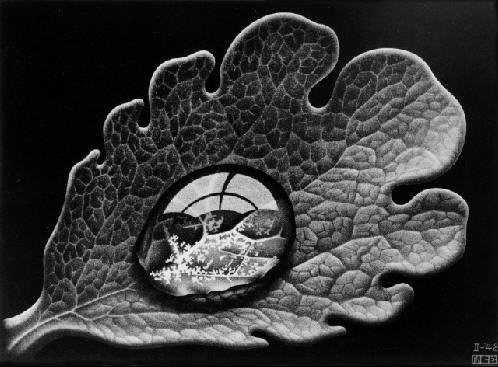
\includegraphics[scale=0.5]{img/dewdrop.eps}
 \captionsetup{labelformat=empty}
 \caption{艾舍尔《露珠》1948}
 \label{fig:Escher-Dewdrop-1948}
\end{wrapfigure}

欢迎来到范畴世界!我建议你小小的奖励自己一下。你已经迈过了第一道门槛,正在通往神奇的抽象王国之路上。这条路是世界上许多最聪明的心智披荆斩棘开辟出来的。如果说,人们将具体的事物,抽象成不带具体意义的数与形是原始阶段;将数、形与计算的意义去除,抽象成代数结构(例如群)和代数关系(例如同构)是第一阶段;范畴可以算是抽象的第二阶段。

你也许会问,什么是范畴?为什么要了解范畴?这和编程有什么关系?范畴是数学家在1940年代研究同调代数时的“副产品”——顺手发明的理论。最近十几年,范畴论由于其强大的抽象,几乎普适于任何问题,正向各种各样的领域渗透。不要说各大编程语言纷纷引入lambda演算和闭包等结构,有超过20种语言已经实现了单子(Monad)\cite{Monad-Haskell-Wiki}——用范畴的语言说,叫做“函子范畴上的幺半群”。许多基本的计算逐渐使用范畴的语言进行抽象\footnote{例如,传统的右侧叠加定义:\\
\texttt{foldr \_ z {[} {]} = z} \\
\texttt{foldr f z (x:xs) = f x (foldr f z xs)} \\
用范畴语言抽象为:\texttt{foldr f z t = appEndo (foldMap (Endo . f) t) z} 详见本章结尾部分。}。

更重要的是:我们需要抽象。赫尔曼$\cdot$外尔说现代数学在过去几十年不断沉湎在抽象和形式化上。编程领域何尝不是如此呢?现代计算机科学解决的问题空前复杂,大数据量、分布式、高并发、还要保证数据和计算的安全。仅仅靠着前几十年的传统方法——暴力求解、务实的工程实践再加上一点聪明的头脑已经不够了。这逼迫着我们去吸取其它科学和数学中的新方法和新工具。

正如迪厄多内所说:“这种抽象绝不是来自数学家的反常意愿,似乎他们想通过使用深奥莫测的语言来把自己与其他人隔开。数学家是被经典对象和关系的本质特性逼着去锻造新的抽象工具,来解决过去看来是不可攻克的问题。”\cite{Dieudonne1987}(中文版第2页,英文版第9页)

范畴论是数学家艾伦伯格和麦克兰恩在1940年代创立的。

\begin{wrapfigure}{R}{0.3\textwidth}
 \centering
 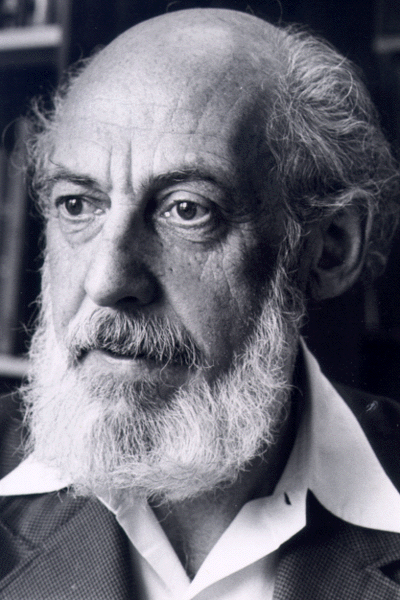
\includegraphics[scale=0.25]{img/Eilenberg.eps}
 \captionsetup{labelformat=empty}
 \caption{艾伦伯格(Samuel Eilenberg, 1913 - 1998)}
 \label{fig:Eilenberg}
\end{wrapfigure}

\index{艾伦伯格}
塞缪尔·艾伦伯格于1913年生于波兰华沙的一个犹太人家庭。父亲是一个酿酒师。他在华沙大学接受了高等教育。当时的华沙大学云集了一批波兰的大数学家,并在点集拓扑学上取得了世界瞩目的成就。他于1936年在华沙大学获得博士学位。在波兰的第二大数学学术中心利沃夫,艾伦伯格结识了著名数学家巴拿赫,并加入了当时著名的数学家团体“苏格兰咖啡”。艾伦伯格和这些数学家们经常聚集在利沃夫市的一家苏格兰咖啡馆,边品尝咖啡边讨论那些没有解决的数学问题。这些未解决的问题后来被整理成了一本书,名叫《苏格兰问题集》(Scottish Book)。1939年,欧洲的局势已经极其紧张。艾伦伯格的父亲劝他移民到美国。他先去了普林斯顿,并于1940年在密歇根大学获得了一个教职。艾伦伯格主要研究代数拓扑。他与诺曼·斯廷罗德(Norman Steenrod)一起对同调理论进行了公理化。艾伦伯格也是著名的布尔巴基小组成员。1949年安德烈·韦伊在芝加哥大学工作的时候邀请艾伦伯格合作编写布尔巴基项目中关于同调群的内容。他与昂利·嘉当合作,在1956年完成了经典著作《同调代数》。艾伦伯格在与麦克兰恩合作研究同调代数的过程中一起创立了范畴论。艾伦伯格后来在纽约哥伦比亚大学做教授,他的主要工作是发展纯粹的范畴论。他是该领域的奠基者之一。1986年他获得沃尔夫奖。1998年艾伦伯格逝世于美国纽约市。

艾伦伯格还是著名的亚洲艺术品收藏家。他收集了来自印度、印度尼西亚、尼泊尔、泰国、柬埔寨、斯里兰卡和中亚的雕塑和艺术品。1992年,他把自己收藏的400多件艺术品捐赠给了纽约大都会博物馆\cite{Wiki-Eilenberg}。

\begin{wrapfigure}{L}{0.3\textwidth}
 \centering
 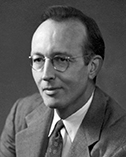
\includegraphics[scale=1]{img/Mac-Lane.eps}
 \captionsetup{labelformat=empty}
 \caption{麦克兰恩(Saunders Mac Lane, 1909 - 2005)}
 \label{fig:Mac-Lane}
\end{wrapfigure}

\index{麦克兰恩}
桑德斯·麦克兰恩1909年生于美国康涅狄格州的诺维奇市。麦克兰恩受洗时的名字是“雷斯利·桑德斯·麦克兰恩”。但是他的父母不喜欢这个名字,所以后来就把雷斯利去掉了。麦克兰恩名字的英文本来是MacLane,他的妻子在打字时总是习惯加上一个空格变成Mac Lane,索性后来麦克兰恩就将错就错了。

麦克兰恩在高中时最喜欢化学。他的父亲在这时去世了,只好由祖父来照顾他。1926年,麦克兰恩的一个远房叔叔资助他到耶鲁学习。他的数学老师希尔带领他参加数学竞赛,并且一路过关斩将获得优胜。从此麦克兰恩下定了从事数学的决心。1930年,麦克兰恩从耶鲁毕业,获得了数学和物理学的双学位。毕业前一年,有一次在新泽西召开耶鲁橄榄球队的球迷聚会。麦克兰恩在会上被授予耶鲁优秀毕业成绩奖\cite{Wiki-Mac-Lane}。恰好芝加哥大学的新任校长哈钦斯也在这次聚会中,他鼓励麦克兰恩到芝加哥大学深造。麦克兰恩于是来到了他后来毕生工作的芝加哥大学\footnote{这里有一段小插曲,聚会后不久,哈钦斯就答应给麦克兰恩一笔奖学金。但是麦克兰恩竟然忘记申请研究生课程就直接去了芝加哥大学。当然最后他被获准入学。}。在芝加哥大学,年近七十岁的数学家摩尔鼓励麦克兰恩前往世界数学圣地——哥廷根大学学习。1931年他获得了硕士学位,接着获得了前往哥廷根大学进修的机会。麦克兰恩幸运的成为了最后一批前往哥廷根的美国人,不久纳粹德国就开始禁止美国人前来学习。

在哥廷根,麦克兰恩师从大数学家保罗$\cdot$伯奈斯、埃米$\cdot$诺特、赫尔曼$\cdot$外尔。在他即将获得博士学位的前夕,导师伯奈斯因为是犹太人,被纳粹政府赶出了校园,于是只好由外尔接替伯奈斯。1934年麦克兰恩获得了哥廷根数学研究所的博士学位,并返回美国\footnote{取得学位后,麦克兰恩与来自芝加哥的多罗茜$\cdot$琼斯结婚(琼斯帮助他打印了博士论文)。他们邀请朋友举行了一个简朴的婚礼。不久后,他们夫妻一起返回了美国。}。

在1944年与1945年,麦克兰恩领导了在第二次世界大战期间有卓越贡献的哥伦比亚大学应用数学小组。麦克兰恩曾任美国科学院与美国哲学会的副主席,美国数学会的主席。在领导美国数学会的期间,他提倡对现代数学教学改进的研习活动。而在1974年至1980年间,他担任了美国政府的科学顾问。1976年,以他为首的美国数学家访问团访问了中国,考察了当时中国数学学术发展。麦克兰恩于1949年获选为美国科学院院士,并在1989年获得美国国家科学奖章。

麦克兰恩的早期研究方向为域论与赋值论。1941年,麦克兰恩在访问密歇根大学时遇到了艾伦伯格。两人开始在代数和拓扑学上进行合作,并结出了累累硕果。1943年,他与艾伦伯格在研究同调代数时一起创立了范畴论。

2005年,麦克兰恩逝世于美国的旧金山。

\section{范畴}

让我们用非洲大草原来了解范畴。在大草原这个范畴中,有很多种动植物。狮子、鬣狗、猎豹、羚羊、水牛、斑马、秃鹫、蜥蜴、眼镜蛇、蚂蚁……我们管这些动物叫做对象,每种动物和植物都是一个对象。这些动植物之间会产生联系,例如狮子会吃羚羊,羚羊吃掉草。我们很容易构造一个食物链。可以从羚羊画一个箭头指向狮子,从草画一个箭头指向羚羊来表示这样的关系。这样对象加上箭头就构成了一个有结构的,彼此联系在一起的系统。

\begin{figure}[htbp]
 \centering
 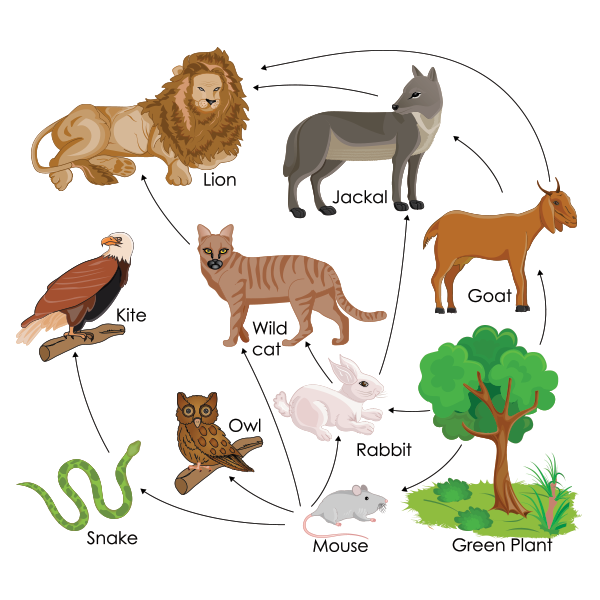
\includegraphics[scale=0.4]{img/food-chain.eps}
 %\captionsetup{labelformat=empty}
 \caption{动植物对象与食物关系箭头组成了一个有结构的系统}
 \label{fig:powerset}
\end{figure}

这样的系统要想成为范畴,还必须满足两点。第一点是每个对象都有指向自己的箭头。这种特殊的箭头称为恒等箭头。对于草原上的动植物,从羚羊到狮子箭头说明羚羊在狮子食物链的下游。我们可以认为每种动植物都处于自己物种食物链的下游(别误会,并不是指吃同类,而是指不吃同类)。这样每个物种就都有自指的箭头了。第二点是箭头之间是可组合的。什么叫做组合呢?草有一个指向羚羊的箭头$f$,羚羊有一个指向狮子的箭头$g$。我们即可以把这两个箭头组合起来成为$g \circ f$,表示草处于狮子食物链的下游。进一步,把两个箭头组合起来后,还可以和第三个箭头再次组合。例如狮子死后会被秃鹫吃掉,这样我们可以从狮子画一个指向秃鹫的箭头$h$。组合在一起就是$h \circ (g \circ f)$。这个箭头的含义表示草处于秃鹫食物链的下游,它等价与$(h \circ g) \circ f$。也就是说,食物链的上下游关系是满足结合性的。

在组合的基础上,还有一个叫作“可交换”的概念。例如下面图中,

\begin{center}
\begin{tikzpicture}
  \matrix (m) [matrix of math nodes,
               row sep=3em, column sep=4em, minimum width=2em]{
     & \text{羚羊} & \\
     \text{草} & & \text{狮子} \\};
  \path[-stealth]
    (m-2-1) edge node [above] {$f$} (m-1-2)
    (m-1-2) edge node [above] {$g$} (m-2-3)
    (m-2-1) edge node [below] {$h$} (m-2-3);
\end{tikzpicture}
\end{center}

可以沿着两条通路从草到达狮子,一条是箭头组合$g \circ f$,表示草在羚羊的下游,羚羊又在狮子的下游;另一条是箭头$h$,表示草在狮子的下游。这样我们就相当于得到了一对平行的箭头:

\begin{center}
\begin{tikzpicture}
  \matrix (m) [matrix of math nodes,
               row sep=3em, column sep=4em, minimum width=2em]{
     \text{草} & \text{狮子} \\};
  \path[-stealth]
    (m-1-1.north east) edge node [above] {$g \circ f$} (m-1-2.north west)
    (m-1-1.south east) edge node [below] {$h$} (m-1-2.south west);
\end{tikzpicture}
\end{center}

如果这两个平行的箭头是等效的,我们称它们是可交换的。用符号表示就是:

\[
h = g \circ f
\]

这样,我们说草原上的动植物,在食物链关系这个箭头下,构成了一个范畴。现在我们给出较为正式的范畴的定义。

\index{范畴} \index{箭头}
\begin{definition}
一个范畴$\pmb{C}$包括一组对象(Object)\footnote{和编程中的“面向对象”无关。这里指抽象事物。},记为$A, B, C, ...$,和一组箭头(Arrow),记为$f, g, h, ...$。它们之上定义了以下四种操作:
\begin{itemize}
\item 两个全操作\footnote{全操作(total operation)是指对于所有的对象,无一例外都存在这一操作。与之相对的是部分操作(partial operation),对于某些对象,这一操作没有定义。例如对于全体整数的集合,取相反数$x \mapsto -x$是全操作,而取倒数$x \mapsto 1/x$由于对0没有定义,所以是部分操作。},称为源(source)和目标(target)\footnote{不应把源和目标理解为名词,而应理解为动词。表示“指定源为……”,“指定目标为……”},这两个操作都将对象指定到箭头上,记为$A \arrowto{f} B$,表示箭头$f$的源是$A$,目标是$B$;
\item 第三个全操作叫恒等箭头\footnote{同样这里恒等箭头(identity arrow)应理解为动词,表示“为……指定恒等箭头”。},对于任何对象$A$,恒等箭头都指向$A$自己。记为:$A \arrowto{id_A} A$;
\item 第四个操作是一个部分操作,称为组合。它将两个箭头组合起来。如果有箭头$B \arrowto{f} C$和$A \arrowto{g} B$,则$f$和$g$的组合为$f \circ g$,读作“$g$然后$f$”。它表示$A \arrowto{f \circ g} C$。
\end{itemize}

除此之外,范畴还必须满足以下两条公理:

\begin{itemize}
\item \textbf{结合性公理}:箭头组合是可结合的。对任何三个可组合的箭头$f, g, h$都有:
\[
f \circ (g \circ h) = (f \circ g) \circ h
\]
我们可以将其写为$f\ g\ h$。
\item \textbf{单位元公理}:恒等箭头对于组合运算来说相当于单位元。
对于任何箭头$A \arrowto{f} B$来说,都有:
\[
f \circ id_A = f = id_B \circ f
\]
\end{itemize}
\end{definition}

和大草原上的食物链比起来,范畴和箭头的定义是很抽象的。我们可以通过一些较为具体的例子,来加深对这个定义的理解。

\subsection{范畴的例子}

在数学上,如果一个集合带有特殊的单位元,元素间定义了可结合的二元运算。我们说这样的集合构成一个幺半群。例如全体整数中,令0是单位元,二元运算是加法,则构成了整数加法幺半群。

幺半群的集合不仅可以包含数,也可以是其它东西。例如英文的词语和句子(在编程中称为字符串)构成一个集合。如果我们把两个英文词句连在一起称为二元运算,例如“red ” $\doubleplus$ “apple” = “red apple”,则这些英文词句构成一个幺半群。其中单位元是空词句“”。不难验证它满足幺半群的条件:

\[
red \doubleplus (apple \doubleplus tree) = (red \doubleplus apple) \doubleplus tree
\]
词句连接满足结合律。

\[
\texttt{""} \doubleplus apple = apple = apple \doubleplus \texttt{""}
\]

任何词句连接上空词句(单位元)都仍然等于它本身。

把词句幺半群放在一边,再考虑另一个幺半群。群元素是字母组成的集合(在编程中称为字符集),二元操作是集合的并,单位元是空集。将两个字母集合并在一起可以获得一个更大的集合,例如:

\[
\{a, b, c, 1, 2\} \cup \{X, Y, Z, 0, 1\} = \{a, b, c, X, Y, Z, 0, 1, 2\}
\]

再加上最初的例子,整数加法幺半群,我们就有三个幺半群了。接下来我们建立这三个幺半群之间的转换关系\footnote{数学上叫做态射(morphism)},首先是从词句幺半群到字母集合幺半群之间的转换关系。任给一个英文词句,我们可以把这句英文中用到的所有不同字母组成一个集合。可以把这个操作叫做“取字母”。可以验证,取字母满足以下条件:

\[
\begin{array}{rcl}
\text{取字母}(red \doubleplus apple) = \text{取字母}(red) \cup \text{取字母}(apple) & \text{和} & \text{取字母}(\texttt{""}) = \varnothing
\end{array}
\]

也就是说,两句英文字词连在一起所涵盖的字母,等于各个字词中字母的并;空串不含有任何字母(空集)。

接下来再定义从字母集合到整数加法幺半群之间的转换关系。任给一个字母集合,我们可以数出它含有多少字母,空集含有0个字母。我们把这个操作叫做“数个数”。

这样就有了两个变换:“取字母”和“数个数”,我们检查一下它们的组合:

\[
\text{词句} \arrowto{\text{取字母}} \text{字母集合} \arrowto{\text{数个数}} \text{整数}
\]

和

\[
\text{词句} \arrowto{\text{数个数} \circ \text{取字母}} \text{整数}
\]

显然组合后“数个数$\circ$取字母”也是一个转换关系。它表示先从英文词句中抽取出不同的字母,然后再统计不同字母的个数。这样,我们就得到了\textbf{幺半群范畴}$\pmb{Mon}$。其中对象是各种各样的幺半群,箭头是彼此间的转换关系,数学上叫做态射。恒等箭头从一个幺半群指向它自己。

这是一个非常巨大的范畴,它包含宇宙中\textbf{所有}的幺半群\footnote{你可能想到了罗素悖论。确切地说,$\pmb{Mon}$包含了宇宙中所有“小”的幺半群}。另一方面,范畴也可以很小,我们接下来看的例子只含有一个幺半群。考虑英文词句这个幺半群,它只有一个对象,就是全体英文的集合(请原谅,这看起来也不怎么小)。对于任何一个英文词句,例如hello,我们都可以定义一个前缀操作,把hello添加到任何其它英文词句前面。我们管这个操作叫“加前缀hello”。例如:“加前缀hello”作用到单词Alice上就变成了helloAlice;类似地还可以定义“加前缀hi”,把它作用到Alice上就得到了hiAlice。如果认为这是两个不同的箭头,则它们的组合就是:

\begin{center}
加前缀hello $\circ$ 加前缀hi = 加前缀hellohi
\end{center}

表示先增加前缀hi,然后再增加前缀hello。不难验证,任意三个这样的箭头满足结合律。接下来我们还需要检查一下单位元,也就是空词句“”。以空词句作为前缀等于没有变化,也就是恒等变换。这样我们就得到了只有一个对象的幺半群范畴,如图\ref{fig:monoid-as-category}所示。

\begin{figure}[htbp]
\centering
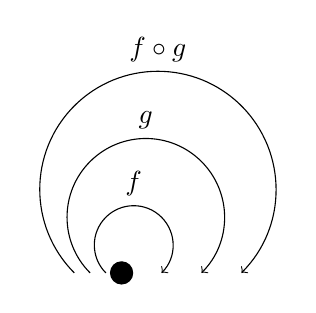
\begin{tikzpicture}
\filldraw (0, 0) circle (4pt) node (obj) {};
\draw[->] (-0.2, 0) arc[radius=5mm, start angle=225, end angle=-45] node[pos=0.5, above]{$f$};
\draw[->] (-0.4, 0) arc[radius=10mm, start angle=225, end angle=-45] node[pos=0.5, above]{$g$};
\draw[->] (-0.6, 0) arc[radius=15mm, start angle=225, end angle=-45] node[pos=0.5, above]{$f \circ g$};
\end{tikzpicture}
\caption{只有一个对象的幺半群范畴}
\label{fig:monoid-as-category}
\end{figure}

\index{幺半群范畴}
同样是幺半群,我们既看到了包含宇宙中全部幺半群的范畴$\pmb{Mon}$,也看到了只包含一个幺半群的范畴。可谓一沙一世界,一花一叶一如来。更有意思的是,对于任何范畴$\pmb{C}$,和其中任何的对象$A$,定义集合$hom(A, A)$为所有从$A$指向$A$的箭头。则这一箭头的集合在组合运算下又构成一个幺半群,其中单位元是恒等箭头。这种对偶值得我们仔细体会。

\index{集合全函数范畴}
我们举的第二个例子是集合。我们让每个集合都成为一个对象\footnote{一旦开始考虑全部集合的集合,就会对导致“全部不包括自身的集合”这样的矛盾,称之为罗素悖论。我们将在第7章详细讲述罗素悖论。},而箭头是从一个集合$A$到另一个集合$B$的函数(或映射)。我们称$A$为函数的定义域,$B$为值域\footnote{确切地说是全函数,即定义域中的每个元素都可以应用的函数}。组合运算就是函数的组合。即$y = f(x)$与$z = g(y)$的组合为$z = (g \circ f)(x) = g(f(x))$。不难验证,函数的组合满足结合律,单位元是恒等函数$id(x) = x$。这样我们就获得了全体集合和函数组成的范畴$\pmb{Set}$。

\index{偏序集} \index{预序集}
我们举的第三个例子包括一对概念。分别叫做\textbf{偏序集}和\textbf{预序集}。给定一个集合,所谓预序(pre-order),是说集合中的两个元素之间可以进行比较。我们用二元关系符号$\leq$来表示,这个符号不一定是大于小于关系,它可能表示一个集合是另一个集合的子集,一个词句是另一个词句的后缀,一个人是另一个人的后代等等。如果关系$\leq$满足以下两条性质,我们说这是一个预序关系:

\begin{itemize}
\item \textbf{自反性}:任何集合中的元素$a$都有$a \leq a$;
\item \textbf{传递性}:若$a \leq b$且$b \leq c$,则$a \leq c$;
\end{itemize}

如果在此基础上还满足反对称性,则这一关系叫做偏序(partial order):

\begin{itemize}
\item \textbf{反对称性}:若$a \leq b$且$b \leq a$,则$a = b$;
\end{itemize}

我们称满足预序关系的集合叫做预序集,满足偏序关系的集合叫做偏序集,分别记作:

\[
preset \quad \quad \quad poset
\]

\begin{figure}[htbp]
\centering
\begin{tikzpicture}[scale=0.5]
  \matrix (m) [matrix of math nodes,
               row sep=1em, column sep=1em, minimum width=2em]{
     & \text{贾演}   & & & & & \text{贾源} & & \\
     & \text{贾代化} & & & & & \text{贾代善} & & \\
     & \text{贾敬}   & & \text{贾赦} & & \text{贾政} & & & \text{贾敏} \\
     \text{贾珍} & \text{贾惜春} & \text{贾迎春} & \text{贾琏} & \text{贾珠} & \text{贾元春} & \text{贾宝玉} & \text{贾探春} & \text{贾环} \\
     \text{贾蓉} & & & \text{巧姐} & \text{贾兰} & & & & & \\};
  \path[<-]
    (m-1-2) edge (m-2-2) %贾演 -- 贾代化
    (m-1-7) edge (m-2-7) %贾源 -- 贾代善
    (m-2-2) edge (m-3-2) %贾代化 -- 贾敬
    (m-2-7) edge (m-3-4) %--贾赦
    (m-2-7) edge (m-3-6) %--贾政
    (m-2-7) edge (m-3-9) %--贾敏
    (m-3-2) edge (m-4-1) %贾敬--贾珍
    (m-3-2) edge (m-4-2) %贾敬--贾惜春
    (m-3-4) edge (m-4-3) %贾赦--贾迎春
    (m-3-4) edge (m-4-4) %贾赦--贾琏
    (m-3-6) edge (m-4-5) %贾政--贾珠
    (m-3-6) edge (m-4-6) %贾政--贾元春
    (m-3-6) edge (m-4-7) %贾政--贾宝玉
    (m-3-6) edge (m-4-8) %贾政--贾探春
    (m-3-6) edge (m-4-9) %贾政--贾环
    (m-4-1) edge (m-5-1) %贾珍--贾蓉
    (m-4-4) edge (m-5-4) %贾琏--巧姐Pre-discuss on OP1 review
    (m-4-5) edge (m-5-5); %贾珠--贾兰
\end{tikzpicture}
\caption{《红楼梦》贾家的家族树}
\label{fig:genealogical-tree}
\end{figure}

在偏序集中,并非任何两个元素都能够进行比较。例如,《红楼梦》中贾家按照祖先关系构成一个偏序集。如果\ref{fig:genealogical-tree}所示。可以看到巧姐$\leq$贾琏,但是贾宝玉和贾探春之间,贾迎春和贾惜春之间无法用$\leq$进行比较。在这棵家族树中,尽管任何人都有祖先(位于树根的人根据自反性,可以认为自己是自己的祖先),但是平辈的人之间无法进行比较。不同枝干上的人之间也无法进行比较。

如图\ref{fig:powerset}所示,一个集合$\{x, y, z\}$的所有子集在包含关系下构成一个偏序集。尽管图中任意元素,都可以找到其子集,但是图中同一层级上的元素间无法比较,另外$\{x\}$和$\{y, z\}$间也无法比较。

\begin{figure}[htbp]
 \centering
 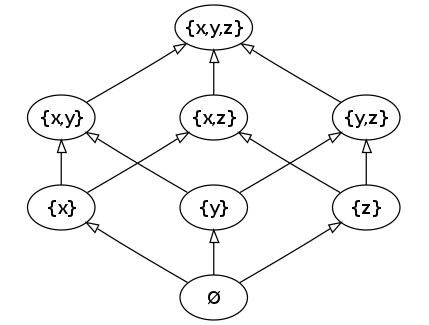
\includegraphics[scale=0.4]{img/powerset.eps}
 %\captionsetup{labelformat=empty}
 \caption{一个集合的子集在包含关系下构成一个偏序集}
 \label{fig:powerset}
\end{figure}

\index{偏序集范畴} \index{预序集范畴}
一般来说,任何一个偏序集都是一个预序集,但是反过来却不一定成立。一个预序集不一定是一个偏序集。高中时我们都学过单调函数,就是那种只增不减的函数,如果$x \leq y$,则$f(x) \leq f(y)$。把这种单调函数组合起来用到偏序集和预序集上,我们就获得了一对范畴

\[
\pmb{Pre} \quad \quad \quad \pmb{Pos}
\]

它们的对象分别是所有的$preset$和$poset$,两个范畴中的箭头都是单调映射。由于恒等映射也是单调映射,所以范畴中的恒等箭头为恒等映射。

幺半群范畴和预序集范畴这两个例子不是随便挑选的,我们有着特殊的用意。这两个范畴可以说是最简单的例子。通过幺半群范畴,我们可以学习组合;通过预序集范畴,我们可以学习比较。对数学结构的组合与比较是整个范畴论的核心。在这一意义上,任何范畴都是幺半群与预序集的某种混合形式(\cite{Simmons2011}第13页)。

$\pmb{Pre}$是包含所有预序集的巨大范畴。另一方面预序集范畴也可以很小。小到只含有一个预序集。考虑一个集合,对象是集合中的元素$i, j, k, ...$。如果$i, j$,可比较并且$i \leq j$,我们就定义箭头

\[
i \longrightarrow j
\]

这样任何对象间或者没有箭头,表示它们不可比较;或者存在一个箭头,表示它们有$\leq$关系。总之,任何两个对象间最多只有一个箭头。可以验证这样定义的箭头可以组合,并且每个元素都有$i \leq i$,因此有指向自己的箭头。这样一个预序集本身就是一个范畴。我们再次看到了预序集范畴和幺半群范畴的对偶。幺半群作为范畴只含有一个对象,却含有丰富的箭头;预序集作为范畴对象很多,但是对象间的箭头却最多只有一个。

\begin{Exercise}
\Question{证明恒等箭头是唯一的(提示:可以参考上一章中群单位元唯一性的证明)。}
\Question{验证幺半群$(S, \cup, \varnothing)$(群元素是集合,二元运算是集合的并,单位元是空集)和$(N, +, 0)$(群元素是自然数,二元运算是加法,单位元是零)都是只含有一个对象的范畴。}
\Question{第一章中我们介绍了自然数的皮亚诺公理,并且介绍了和皮亚诺算术同构的其它结构,例如链表等。这些完全可以用范畴来解释。这一结论是德国数学家戴德金发现的,尽管当时还没有范畴论。我们今天将这一范畴命名为皮亚诺范畴$\pmb{Pno}$。范畴中的对象为$(A, f, z)$,其中$A$为元素的集合,对于自然数来说这个集合是全体自然数$N$;$f: A \to A$是后继函数,对于自然数来说,就是$succ$;$z \in A$是起始元素,对于自然数来说是0。任给两个皮亚诺对象$(A, f, z)$和$(B, g, c)$,现在定义从$A$到$B$的态射
\[
A \arrowto{\phi} B
\]
它满足

\[
\phi \circ f = g \circ \phi \quad \text{且} \quad \phi(z) = c
\]

试验证$\pmb{Pno}$的确是一个范畴。}
\end{Exercise}

\subsection{箭头$\neq$函数}

在此前的例子中,箭头要么是一般意义上的函数,要么是类似函数意义的映射和态射。这容易造成一种错觉,认为箭头等同于函数。我们接下来看的例子有助于打破这种错觉。有一种名叫关系的范畴。范畴中的对象是集合。从集合$A$到$B$的箭头$A \arrowto{R} B$的定义为:

\[
R \subseteq B \times A
\]

我们来看看这个箭头的含义是什么。集合$B \times A$代表了所有$B$和$A$中元素对的组合。也叫做$B$和$A$的积:

\[
B \times A = \{(b, a) | b \in B, a \in A\}
\]

我们以红楼梦人物为例,集合$A =$ \{贾蓉, 贾惜春, 贾琏\},集合$B =$ \{秦可卿, 王熙凤\},则$B \times A$的积为\{(秦可卿, 贾蓉), (秦可卿, 贾惜春), (秦可卿, 贾琏), (王熙凤, 贾蓉), (王熙凤, 贾惜春), (王熙凤, 贾琏)\}。集合$R$是$B \times A$的子集,它可以看作$A$与$B$的某种关系。如果$A$中的元素$a$和$B$中的元素$b$满足关系$R$,则有$(b, a) \in R$,我们将其记为$bRa$。具体到这个例子,我们令$R=$\{(秦可卿, 贾蓉), (王熙凤, 贾琏)\},则$R$代表婚姻关系。

这样从对象$A$到$B$的\textbf{所有}箭头构成的集合就代表了从$A$到$B$的各种可能的关系。现在我们考虑箭头的组合

\[
A \to B \to C
\]

如果存在某个中间集合中的元素$b$,同时使得两个关系$bRa$,$cSb$都成立,我们就说存在箭头间的组合。具体到红楼梦的例子,令集合$C=$\{王夫人, 薛姨妈, 邢夫人\},关系$S=$\{(王夫人, 王熙凤), (薛姨妈, 王熙凤)\}表示姑妈关系。这样组合箭头$S \circ R$的结果是:\{(王夫人, 贾琏), (薛姨妈, 贾琏)\},表示$c$的侄女嫁给了$a$的关系。也就是说王夫人、薛姨妈和贾琏都通过王熙凤使得两个关系同时成立。恒等箭头的定义很简单,所有元素都和自己产生恒等关系。

我们还可以从任何已知的范畴产生新的范畴,例如把一个范畴$\pmb{C}$中的所有箭头反向就得到了一个对偶的范畴$\pmb{C}^{op}$。这样我们了解了一个范畴,就同时了解了它的对偶范畴。

\section{函子}
我们说范畴论是对抽象代数结构的“二次抽象”。上一节我们看到如何把所有的集合和映射、群和态射、偏序集和单调函数等抽象成范畴。接下来的问题是,如何在这些范畴之间架设桥梁、进行比较?函子\footnote{C++语言的一些资料中,用英文functor来命名函数对象,即function object。这与范畴论中的函子完全无关。}(functor)就是用来对范畴及其内在的关系(对象和箭头)进行比较的。

\subsection{函子的定义}
\index{函子}
在某种意义上说,函子好比是范畴之间的变换关系(态射)。但是它不仅把一个范畴中的对象映射为另一范畴中的对象,它还将一个范畴中的箭头映射到另一个范畴中。这一点是和普通的态射(例如群之间的态射)不同的。

函子通常用符号$\mathbf{F}$表示。既然说函子好比是范畴间的态射,那么函子必须能够忠实保持范畴间的结构和关系,这是如何做到的呢?为此函子必须满足两条性质。

\begin{itemize}
\item 第一条性质,是函子必须保持恒等箭头仍然变换为恒等箭头。用图来表示就是:

\[
A \arrowto{id} A \quad \longmapsto \quad \mathbf{F}A \arrowto{id} \mathbf{F}A
\]

\index{协变} \index{反变}
\item 第二条性质,函子必须能够保持箭头的组合仍然变换为箭头的组合\footnote{实际存在两种变换方式,一种叫做协变,一种叫做反变(在编程语言的类型系统中译为“逆变”。编程语言借鉴了范畴论中函子相关的用语)。这里仅考虑了协变。}。

\begin{center}
\begin{tikzpicture}
  \matrix (m) [matrix of math nodes,
               row sep=2em, column sep=2.5em, minimum width=2em]{
       & B &   & \longmapsto &             & \mathbf{F}B & \\
     A &   & C & \text{协变} & \mathbf{F}A &  & \mathbf{F}C\\};
  \path[-stealth]
    (m-2-1) edge node [above] {$f$} (m-1-2)
    (m-1-2) edge node [above] {$g$} (m-2-3)
    (m-2-1) edge node [below] {$g \circ f$} (m-2-3)
    (m-2-5) edge node [above] {$\mathbf{F}(f)$} (m-1-6)
    (m-1-6) edge node [above] {$\mathbf{F}(g)$} (m-2-7)
    (m-2-5) edge node [below] {$\mathbf{F}(g \circ f)$} (m-2-7);
\end{tikzpicture}
\end{center}

\[
\mathbf{F}(g \circ f) = \mathbf{F}(g) \circ \mathbf{F}(f)
\]
\end{itemize}

函子之间也可以进行组合,例如函子$(\mathbf{F} \mathbf{G})(f)$表示先用函子$\mathbf{G}$对箭头$f$进行变换,然后再用$\mathbf{F}$对这一新范畴中的箭头进行变换。

\subsection{函子的例子}
\label{sec:functor:examples}

\begin{wrapfigure}{R}{0.3\textwidth}
 \centering
 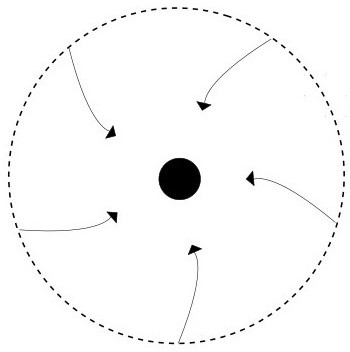
\includegraphics[scale=0.3]{img/blackhole.eps}
 \captionsetup{labelformat=empty}
 \caption{常数函子的行为像一个黑洞}
 \label{fig:blackhole}
\end{wrapfigure}

\index{函子!恒等函子} \index{函子!id函子}
让我们用具体的例子来更好地理解函子的概念。如果一个函子从一个范畴映射到这个范畴本身上,这样的函子被称为\textbf{自函子}(endo-functor)\footnote{这和代数中的自同构概念很类似。如果记不清了,请回顾一下上一章。}。最简单的函子称为“恒等函子”,它是一个自函子,记为$id: \pmb{C} \to \pmb{C}$。它可以作用到任何范畴上,将对象$A$映射为对象$A$,将箭头$f$映射为箭头$f$。

\index{函子!常函子}
其次简单的函子叫做“常函子”,它的行为像一个黑洞,我们可以把它记作$\mathbf{K}_B : \pmb{C} \to \pmb{B}$。它可以作用到任何范畴上,把所有的对象都映射为黑洞中的对象$B$,把所有的箭头都映射为黑洞中的恒等箭头$id_B$。黑洞范畴中只有一个恒等箭头,它显然也满足箭头组合的性质:$id_B \circ id_B = id_B$。

\begin{example}
\index{函子!可能函子} \index{函子!Maybe函子}
我们接下来举的例子叫做“可能函子”(maybe functor)。计算机科学家,快速排序算法的提出者,1980年图灵奖得主霍尔\footnote{英文是Hoare,不是美国物理学家霍尔(Hall)。}曾说过一段有趣的话\footnote{2009年在伦敦举行的QCon会议上}。

%\begin{wrapfigure}{L}{0.25\textwidth}
\begin{figure}[htbp]
 \centering
 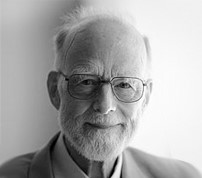
\includegraphics[scale=1]{img/Hoare.eps}
 \captionsetup{labelformat=empty}
 \caption{计算机科学家霍尔}
 \label{fig:Hoare}
\end{figure}
%\end{wrapfigure}

“我在1965年发明了空引用(null reference)。这是一个导致数十亿美元损失的发明。当时,我在为一种面向对象语言(ALGOL W)设计最早的类型系统。我希望能够保证所有的引用,经过编译器的自动检查,都是绝对安全的。但是我无法抗拒空引用的想法,它太容易实现了。此后,空引用导致了无数的错误、漏洞和系统崩溃。在过去的40年,由此导致的痛苦损失估计高达数十亿美元。”\cite{Wiki-Hoare}

% I call it my billion-dollar mistake. It was the invention of the null reference in 1965. At that time, I was designing the first comprehensive type system for references in an object oriented language (ALGOL W). My goal was to ensure that all use of references should be absolutely safe, with checking performed automatically by the compiler. But I couldn't resist the temptation to put in a null reference, simply because it was so easy to implement. This has led to innumerable errors, vulnerabilities, and system crashes, which have probably caused a billion dollars of pain and damage in the last forty years.

2015年后主流的编程环境都纷纷将Maybe概念引入以取代null来获取更安全的方法\footnote{例如Java和C++中的\texttt{Optional<T>}。}。

下图描述了$\mathbf{Maybe}$函子的行为。

\begin{center}
\begin{tikzpicture}
  \matrix (m) [matrix of math nodes,
               row sep=2em, column sep=2.5em, minimum width=2em]{
     A & \mathbf{Maybe}\ A \\
     B & \mathbf{Maybe}\ B \\};
  \path[-stealth]
    (m-1-1) edge (m-1-2)
    (m-2-1) edge (m-2-2)
    (m-1-1) edge node [left] {$f$} (m-2-1)
    (m-1-2) edge node [right] {$\mathbf{Maybe}(f)$} (m-2-2);
\end{tikzpicture}
\end{center}

图中左侧的对象$A, B$是一些数据类型,比如整形,布尔型。而右侧的对象,是通过函子$\mathbf{Maybe}$映射成的类型。如果$A$代表$Int$,则右侧对应是$\mathbf{Maybe}\ Int$,$B$如果代表$Bool$,则右侧对应的是$\mathbf{Maybe}\ Bool$。可能函子是怎样完成对象的映射呢?它的对象映射部分是这样定义的:

\lstset{frame=none}
\begin{lstlisting}
data Maybe A = Nothing | Just A
\end{lstlisting}

也就是说,若对象是类型$A$,则映射到的对象是类型$\mathbf{Maybe}\ A$。注意,这里的对象是类型,而不是值。而类型$\mathbf{Maybe}\ A$的值要么是一个空值$Nothing$,要么是一个用$Just$构造的值。

例如,对象是类型$Int$,可能函子映射后对象是类型$\mathbf{Maybe}\ Int$,它的值可能是$Nothing$或者$Just\ 5$。

例如有一个元素类型为$A$的二叉搜索树,在其中搜索一个值时,可能会搜不到。所以搜索的结果类型是$\mathbf{Maybe}\ A$\footnote{完整的代码见本章附录}。

\[
\begin{array}{rcl}
lookup\ Nil\ \_ & = & Nothing \\
lookup\ (Br\ l\ k\ r)\ x & = & \begin{cases}
  x < k: & lookup\ l\ x \\
  x > k: & lookup\ r\ x \\
  x = k: & Just\ k
\end{cases}
\end{array}
\]

在处理$\mathbf{Maybe}$数据类型时,必须处理可能的两种值,例如:

\[
\begin{array}{lcl}
elem\ Nothing & = & False \\
elem\ (Just\ x) & = & True
\end{array}
\]

函子既映射对象,也映射箭头。以上我们看到了$\mathbf{Maybe}$如何映射对象,那么它是如何映射箭头的呢?上面图中的左侧从上到下有一个箭头$A \arrowto{f} B$,而右侧也有一个箭头$\mathbf{Maybe}\ A \arrowto{\mathbf{Maybe}(f)} \mathbf{Maybe}\ B$。我们不妨把右侧的箭头叫做$f'$。假设我们知道左侧箭头$f$的行为,那么右侧箭头的行为是什么呢?我们说过处理$\mathbf{Maybe}$类型的数据,必须处理两种可能的值,所以$f'$的行为应该是这样的:

\[
\begin{array}{lcl}
f'\ Nothing & = & Nothing \\
f'\ (Just\ x) & = & Just\ (f\ x)
\end{array}
\]

\index{fmap}
这种给定$f$,映射成$f'$的行为恰好就是$\mathbf{Maybe}$函子对箭头进行的映射。实际的编程环境中,通常使用$fmap$来定义函子对箭头的映射。我们可以定义所有函子$\mathbf{F}$满足:

\[
fmap : (A \to B) \to (\mathbf{F} A \to \mathbf{F} B)
\]

也就是说,如果$\mathbf{F}$是一个函子,它把从$A$到$B$的箭头映射成从$\mathbf{F} A$到$\mathbf{F} B$的箭头。因此对于$\mathbf{Maybe}$函子,相应的$fmap$定义如下:

\[
\begin{array}{l}
\quad    fmap : (A \to B) \to (\mathbf{Maybe}\ A \to \mathbf{Maybe}\ B) \\
\quad    fmap\ f\ Nothing = Nothing \\
\quad    fmap\ f\ (Just\ x) = Just\ (f\ x) \\
\end{array}
\]

回到前面二叉搜索树的例子,假如树中元素的类型是自然数,我们在树中搜索一个值,如果搜到,就将这个值转换成二进制,否则返回$Nothing$。如果我们以前已经写过一个将十进制自然数转换成二进制的函数:

\[
binary(n) = \begin{cases}
n < 2: & [n] \\
\text{否则}: & binary(\lfloor\dfrac{n}{2}\rfloor)\doubleplus[n \bmod 2]
\end{cases}
\]

下面是一个相应的例子代码实现。为了提高性能,这个实现使用了尾递归。

\lstset{frame=single}
\begin{lstlisting}[style=Haskell]
binary = bin [] where
   bin xs 0 = 0 : xs
   bin xs 1 = 1 : xs
   bin xs n = bin ((n `mod` 2) : xs) (n `div` 2)
\end{lstlisting}

有了函子,就可以直接将这个函数箭头“举”到上面去,如下图所示:

\begin{center}
\begin{tikzpicture}
  \matrix (m) [matrix of math nodes,
               row sep=2em, column sep=6em, minimum width=2em]{
     \mathbf{Maybe}\ Int & \mathbf{Maybe}\ [Int] \\
     Int & \left [ Int \right] \\};
  \path[-stealth]
    (m-1-1) edge node [above] {$fmap\ binary$} (m-1-2)
    (m-2-1) edge node [below] {$binary$} (m-2-2)
    (m-2-1) edge (m-1-1)
    (m-2-2) edge (m-1-2);
\end{tikzpicture}
\end{center}

这样,我们就可以直接利用Maybe函子和$binary$箭头操作二叉树搜索的结果:

\[
fmap\ binary\ (lookup\ t\ x)
\]

\begin{mdframed}
\begin{proof}
\textbf{一般的读者可以跳过这个框中的内容。}为了验证Maybe的确是一个函子,我们还需要验证箭头映射的两条性质:

\[
\begin{array}{l}
fmap\ id = id \\
fmap\ (f \circ g) = fmap\ f \circ fmap\ g
\end{array}
\]

首先验证第一条性质。$id$的定义为:
\[
id\ x = x
\]

因此:

\[
\begin{array}{rcll}
fmap\ id\ Nothing & = & Nothing & \text{$fmap$的定义} \\
                  & = & id\ Nothing & \text{反向用$id$的定义} \\
\end{array}
\]

并且

\[
\begin{array}{rcll}
fmap\ id\ (Just\ x) & = & Just\ (id\ x) & \text{$fmap$的定义} \\
                    & = & Just\ x & \text{$id$的定义} \\
                    & = & id\ (Just\ x) & \text{反向用$id$的定义}
\end{array}
\]

接下来验证第二条性质:

\[
\begin{array}{rcll}
fmap\ (f \circ g)\ Nothing & = & Nothing & \text{$fmap$的定义} \\
           & = & fmap\ f\ Nothing & \text{反向使用$fmap$的定义} \\
           & = & fmap\ f\ (fmap\ g\ Nothing) & \text{反向使用$fmap$的定义} \\
           & = & (fmap\ f\ \circ fmap\ g)\ Nothing & \text{反向用函数组合的定义}
\end{array}
\]

并且

\[
\begin{array}{rcll}
fmap\ (f \circ g)\ (Just\ x) & = & Just\ ((f \circ g)\ x) & \text{$fmap$的定义} \\
           & = & Just\ (f\ (g\ x)) & \text{函数组合的定义} \\
           & = & fmap\ f\ (Just\ (g\ x)) & \text{反向使用$fmap$的定义} \\
           & = & fmap\ f\ (fmap\ g\ (Just\ x)) & \text{反向使用$fmap$的定义} \\
           & = & (fmap\ f\ \circ fmap\ g)\ (Just\ x) & \text{反向用函数组合的定义}
\end{array}
\]

因此Maybe的确是一个函子。
\end{proof}
\end{mdframed}
\end{example}

\begin{example}
\index{函子!列表函子}
接下来介绍的例子是列表函子。在第一章中我们介绍了列表的定义:

\lstset{frame=none}
\begin{lstlisting}
data List A = Nil | Cons(A, List A)
\end{lstlisting}

从编程的观点看,这定义了“单向链表”的数据结构,链表中元素的类型是$A$,这样的链表称为类型为$A$的列表。从范畴的观点来看,一个列表函子要分别定义对象和箭头的映射。在这里,对象是类型,箭头是全函数。下图描述了列表函子的行为:

\begin{center}
\begin{tikzpicture}
  \matrix (m) [matrix of math nodes,
               row sep=2em, column sep=2.5em, minimum width=2em]{
     A & \mathbf{List}\ A \\
     B & \mathbf{List}\ B \\};
  \path[-stealth]
    (m-1-1) edge (m-1-2)
    (m-2-1) edge (m-2-2)
    (m-1-1) edge node [left] {$f$} (m-2-1)
    (m-1-2) edge node [right] {$\mathbf{List}(f)$} (m-2-2);
\end{tikzpicture}
\end{center}

图中左侧的对象$A, B$是数据类型,例如整型、布尔型甚至是$\mathbf{Maybe}\ Char$这样的复杂类型。而右侧的对象,是通过列表函子映射成的类型,如果$A$为整形$Int$,则右侧对应$\mathbf{List}\ Int$,如果$B$代表$Char$,则右侧对应的是$\mathbf{List}\ Char$,也就是$String$。

请再次注意这里的对象是类型,而不是值,$A$可以是$Int$,但不是具体的值5。因此$\mathbf{List}\ A$对应整形列表,是一个类型,而不是一个具体的值,如:[1, 1, 2, 3, 5]。那么如何产生具体的列表值呢?那要靠$Nil$和$Cons$两个具体的函数来产生空值或者诸如$List(1, List(1, List(2, Nil)))$这样的具体列表。

以上是列表函子在对象映射时的行为,那么它是如何对箭头进行映射的呢?也就是说,给定一个函数$f: A \to B$,如何通过列表函子得到另一个函数$g: \mathbf{List}\ A \to \mathbf{List}\ B$呢?与可能函子$\mathbf{Maybe}$类似,我们可以定义一个$fmap$实现从箭头$f$到箭头$g$的映射,对于列表函子它的类型为:

\[
fmap: (A \to B) \to (\mathbf{List}\ A \to \mathbf{List}\ B)
\]

接下来需要仔细分析$g$的行为。首先考虑最简单的情况,不管箭头$f$的定义如何,如果$\mathbf{List}\ A$是个空列表$Nil$,则应用$g$后的结果也必然是空列表。所以有:

\[
fmap\ f\ Nil = Nil
\]

接下来考虑递归的情况$Cons(x, xs)$,其中$x$是类型为$A$的某个值,而$xs$是类型为$\mathbf{List}\ A$的子列表。如果$f(x) = y$,将类型$A$的值$x$映射为类型$B$的值$y$,那么我们就将$f$应用到$x$上,然后在将其递归地应用到子列表$xs$上从而得到一个元素类型为$B$的子列表$ys$,最后再将$y$和$ys$链接起来得到最终的结果:

\[
fmap\ f\ Cons(x, xs) = Cons(f\ x, fmap\ f\ xs)
\]

综上,我们得到了$fmap$的完整定义:

\[
\begin{array}{l}
\quad    fmap : (A \to B) \to (\mathbf{List}\ A \to \mathbf{List}\ B) \\
\quad    fmap\ f\ Nil = Nil \\
\quad    fmap\ f\ Cons(x, xs) = Cons(f\ x, fmap\ f\ xs) \\
\end{array}
\]

如果使用第一章介绍的简记法,用冒号“:”表示$Cons$,用中括号表示列表,用“[]”表示$Nil$,则列表函子的箭头部分映射可以简写为:

\[
\begin{array}{l}
\quad    fmap : (A \to B) \to (\mathbf{List}\ A \to \mathbf{List}\ B) \\
\quad    fmap\ f\ [] = [] \\
\quad    fmap\ f\ (x:xs) = (f\ x):(fmap\ f\ xs) \\
\end{array}
\]

仔细观察这个定义,再和第一章中列表的“逐一映射”定义对比,会发现它们除了名字之外完全一样,因此我们可以复用列表的“逐一映射”来定义列表函子,在一些编程环境中,列表函子的定义就是通过复用\texttt{map}实现的。

\lstset{frame=single}
\begin{lstlisting}
instance Functor [] where
    fmap = map
\end{lstlisting}

作为本例的结尾,我们来验证一下列表函子的箭头映射部分是否满足组合和恒等的两条性质。\textbf{一般的读者可以跳过这一证明部分}。

\begin{mdframed}
\[
\begin{array}{l}
fmap\ id = id \\
fmap\ (f \circ g) = fmap\ f \circ fmap\ g
\end{array}
\]

\begin{proof}
我们用数学归纳法来验证恒等性质,首先针对空列表的情况:

\[
\begin{array}{rcll}
fmap\ id\ Nil & = & Nil & \text{$fmap$的定义} \\
              & = & id\ Nil & \text{反向用$id$的定义} \\
\end{array}
\]

针对$(x:xs)$的递归情况,令递归假设为$fmap\ id\ xs = id\ xs$,我们有:

\[
\begin{array}{rcll}
fmap\ id\ (x:xs) & = & (id\ x):(fmap\ id\ xs) & \text{$fmap$的定义} \\
                 & = & (id\ x):(id\ xs) & \text{递归假设} \\
                 & = & x:xs & \text{$id$的定义} \\
                 & = & id\ (x:xs) & \text{反向用$id$的定义}
\end{array}
\]

同样,我们用数学归纳法来验证组合性质,对于空列表,我们有:

\[
\begin{array}{rcll}
fmap\ (f \circ g)\ Nil & = & Nil & \text{$fmap$的定义} \\
           & = & fmap\ f\ Nil & \text{反向使用$fmap$的定义} \\
           & = & fmap\ f\ (fmap\ g\ Nil) & \text{反向使用$fmap$的定义} \\
           & = & (fmap\ f\ \circ fmap\ g)\ Nil & \text{反向用函数组合的定义}
\end{array}
\]

针对$(x:xs)$的递归情况,令递归假设为$fmap\ (f \circ g)\ xs = (fmap\ f \circ fmap\ g)\ xs$,我们有:

\[
\begin{array}{rcll}
fmap\ (f \circ g)\ (x:xs) & = & ((f \circ g)\ x):(fmap\ (f \circ g)\ xs) & \text{$fmap$的定义} \\
  & = & ((f \circ g)\ x):((fmap\ f \circ fmap\ g)\ xs) & \text{递归假设} \\
  & = & (f(g\ x)):(fmap\ f\ (fmap\ g\ xs)) & \text{函数组合的定义} \\
  & = & fmap\ f\ ((g\ x):(fmap\ g\ xs)) & \text{反向使用$fmap$的定义} \\
  & = & fmap\ f\ (fmap\ g\ (x:xs)) & \text{再次反向使用$fmap$的定义} \\
  & = & (fmap\ f\ \circ fmap\ g)\ (x:xs) & \text{反向用函数组合的定义}
\end{array}
\]

这就验证了$\mathbf{List}$的确是一个函子。
\end{proof}
\end{mdframed}
\end{example}

\begin{Exercise}
\Question{请使用叠加操作$foldr$来定义列表函子的箭头映射。}
\Question{证明可能函子和列表函子的组合$\mathbf{Maybe} \circ \mathbf{List}$与$\mathbf{List} \circ \mathbf{Maybe}$仍然是函子。}
\Question{证明任意函子的组合$\mathbf{G} \circ \mathbf{F}$仍然是函子。}
\Question{思考一个预序集范畴上的函子的例子。}
\Question{回顾第二章中介绍的二叉树,请定义一个二叉树函子。}
\end{Exercise}

\section{积和余积}

在介绍更复杂的范畴和函子的例子之前,我们先了解一下积和余积的概念。这里的积是指范畴的积。为了容易理解,我们先从集合的积入手。两个集合$A$和$B$的笛卡尔积$A \times B$,是所有有序对$(a, b)$的集合。其中$a \in A, b \in B$。即:

\[
\{(a, b) | a \in A, b \in B\}
\]

例如有限集合$\{1, 2, 3\}$和$\{a, b\}$的积为

\[
\{(1, a), (2, a), (3, a), (1, b), (2, b), (3, b)\}
\]

如果集合$A, B$是同类的代数结构,如群、环等,我们可以定义如下图的对象和箭头。

\begin{center}
\begin{tikzpicture}
  \matrix (m) [matrix of math nodes,
               row sep=2em, column sep=2em, minimum width=2em]{
      &   & (a, b) &  & \\
      &   & A \times B & & \\
      &   &            & & \\
    a & A &            & B & b \\};
  \path[|->]
    (m-1-3) edge (m-4-1)
    (m-1-3) edge (m-4-5);
  \path[-stealth]
    (m-2-3) edge (m-4-2)
    (m-2-3) edge (m-4-4);
\end{tikzpicture}
\end{center}

%\begin{wrapfigure}{L}{0.25\textwidth}
\begin{figure}[htbp]
 \centering
 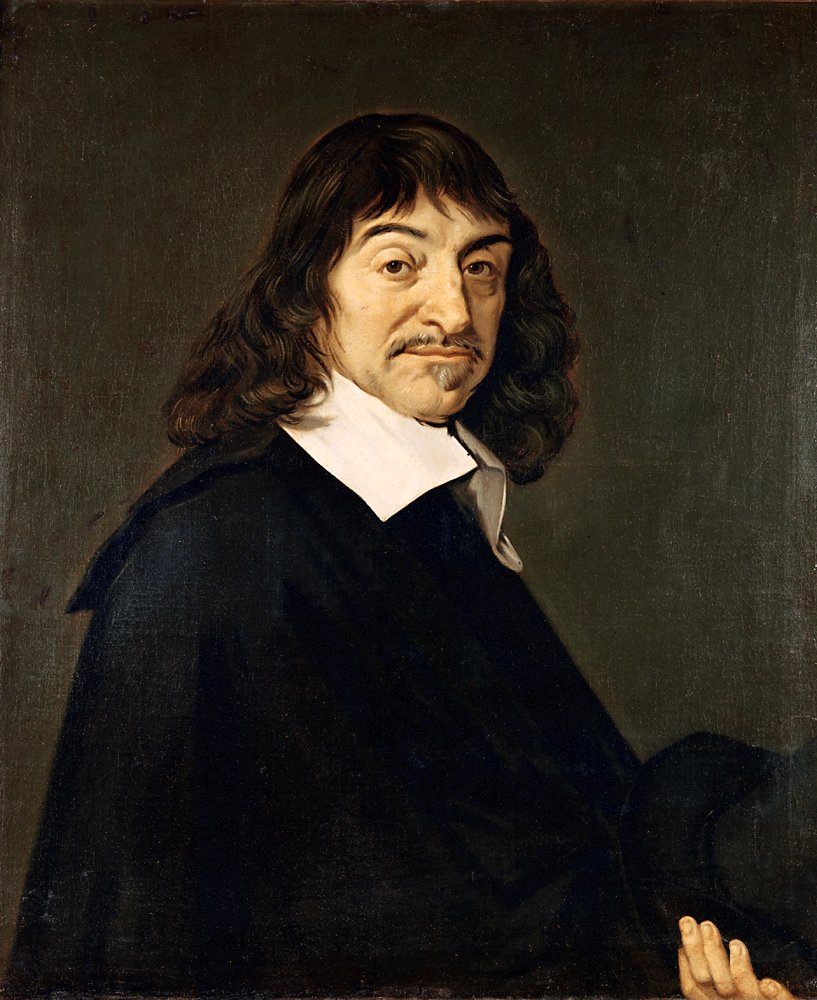
\includegraphics[scale=0.2]{img/Descartes.eps}
 \captionsetup{labelformat=empty}
 \caption{勒内$\cdot$笛卡尔(1596-1650)。哈尔斯的画布油画,现藏于卢浮宫}
 \label{fig:Decartes}
\end{figure}
%\end{wrapfigure}

\index{笛卡尔积} \index{笛卡尔}
笛卡尔积又称直积,是用法国哲学家、数学家、物理学家笛卡尔的名字命名的。在笛卡尔的时代,拉丁文是学术上广泛使用的语言。笛卡尔也有一个拉丁化的名字——卡提修斯(Cartesius)。正因为如此,笛卡尔积也称卡氏积,笛卡尔坐标系也称卡氏坐标系。

笛卡尔1596年生于法国一个地位较低的贵族家庭。一岁时他的母亲患肺结核去世,而他也受到传染,造成体弱多病。母亲去世后,父亲移居他乡并再婚,笛卡尔由外祖母带大,自此父子很少见面,但是父亲一直提供金钱方面的帮助,使他能够受到良好的教育。

笛卡尔后来进入位于拉弗莱什的耶稣会的皇家大亨利学院学习。在那里,他学习到了数学和物理学,包括伽利略的工作。由于笛卡尔体弱多病,学校特许他每天早上不用像其他同学一样5点起床,而是一直睡到11点。笛卡尔直到晚年仍然保留了这一作息习惯。

1614年毕业后,他遵从父亲的意愿,进入普瓦捷大学学习法律,并获得业士学位和文凭。毕业后笛卡尔一直对职业选择不定,又决心游历欧洲各地,专心寻求“世界这本大书”中的智慧。1618年,笛卡尔加入荷兰的拿骚的毛里茨的军队。

笛卡尔对结合数学与物理学的兴趣,是在荷兰当兵期间产生的。1618年,他偶然在路旁公告栏上,看到用佛莱芒语提出的数学问题征答。这引起了他的兴趣,并且让身旁的人,将他不懂的佛莱芒语翻译成拉丁语。这位身旁的人就是大他八岁的以撒·贝克曼(Isaac Beeckman)。贝克曼在数学和物理学方面有很高造诣,很快成为了他的导师。4个月后,他写信给贝克曼:“你是将我从冷漠中唤醒的人……”。

1622年,当他26岁时,笛卡尔变卖掉父亲留下的资产,用4年时间游历欧洲。他先在意大利住了2年,随后迁往于巴黎。当时法国教会势力庞大,不能自由讨论宗教问题,因此笛卡尔在1628年移居荷兰,在那里住了20多年。他深居简出,仅仅通过好友梅森\footnote{马林$\cdot$梅森,法国修道士、学者、数学家和音乐理论家。他发现了梅森素数,即形如$M_n = 2^n − 1$的素数。他和当时的著名数学家和科学家有广泛的联系,被称为16世纪上半叶世界数学和科学的中心人物。}和学术界取得联系。在此期间,笛卡尔致力于哲学研究,他发表了多部重要的文集,包括《方法论》、《形而上学的沉思》和《哲学原理》等,成为欧洲最有影响力的哲学家之一。1637年,笛卡尔在他的文章《几何学》中,创立了解析几何。

1649年笛卡尔受瑞典克里斯蒂娜女王之邀来到斯德哥尔摩担任女王的私人教师。但是女王习惯在清晨5点起床向笛卡尔学习,这一下子打破了笛卡尔一生11点起床的作息习惯。几个月后,在这片“熊、冰雪与岩石的土地”上,笛卡尔不幸得了肺炎,在1650年2月去世,享年54岁。

笛卡尔留下名言“我思故我在”,提出了“普遍怀疑”的主张。他开拓了欧洲理性主义哲学,是西方现代哲学的奠基人。他的哲学思想深深影响了之后的几代人。笛卡尔对现代数学的发展做出了重要的贡献,他创立的解析几何,成功地将当时完全分开的代数和几何学联系到了一起。

\vspace{5mm}

相对于集合的笛卡尔积,还有一种对偶的构造。我们可以从两个集合$A, B$产生一个不相交的并集(disjoint union,也称为和)$A + B$。为了分清和中的每个元素究竟是来自$A$还是$B$,可以给元素增加一个标记(tag):

\[
A + B = (A \times \{0\}) \cup (B \times \{1\})
\]

当从$A+B$中取出一个元素$(x, tag)$,如果$tag$为0,我们就知道$x$本来属于$A$,如果$tag$为1,就知道$x$本来属于$B$。这样有限集合$\{1, 2, 3\}$和$\{a, b\}$的和就是

\[
\{(1, 0), (2, 0), (3, 0), (a, 1), (b, 1)\}
\]

$A + B$也可以用程序等价地这样定义:

\begin{mdframed}
\[
A + B = zip\ A\ \{0, ...\} \doubleplus zip\ B\ \{1, ...\}
\]
\end{mdframed}


当$A, B$是同类的代数结构时,我们可以定义如下的对象和箭头:

\begin{center}
\begin{tikzpicture}
  \matrix (m) [matrix of math nodes,
               row sep=2em, column sep=2em, minimum width=2em]{
    a & A &        &       &        & B & b \\
      &   &        &       &        &   & \\
      &   & (a, 0) & A + B & (b, 1) &   & \\};
  \path[|->]
    (m-1-1) edge (m-3-3)
    (m-1-7) edge (m-3-5);
  \path[-stealth]
    (m-1-2) edge (m-3-4)
    (m-1-6) edge (m-3-4);
\end{tikzpicture}
\end{center}

%\begin{wrapfigure}{R}{0.4\textwidth}
\begin{figure}[htbp]
 \centering
 
\includegraphics[scale=0.06]{img/hands.eps}
 \captionsetup{labelformat=empty}
 \caption{}
 \label{fig:hands}
\end{figure}
%\end{wrapfigure}

对比这两种构造我们发现它们是对偶的。如果把两张图旋转90度,把$A$画在上面,$B$画在下面,这样两个问题一个在左侧,一个在右侧。如同双手一样对称。我们后面会发现,这种现象在范畴的相关概念中很常见。甚至我们的宇宙中也充满了对称。这样当我们了解了一个事物,就对偶地了解了另一个事物。

\subsection{积和余积的定义}
\index{积} \index{余积}
\begin{definition}
对于范畴$\pmb{C}$中的一对对象$A$和$B$,一个

\[
\text{指向$A, B$的} \quad \quad \quad \text{从$A, B$出发的}
\]

\index{楔形(wedge)}
\textbf{楔形}(wedge)是范畴$\pmb{C}$中的一个对象$X$和一对箭头:

\begin{center}
\begin{tikzpicture}
  \matrix (m) [matrix of math nodes,
               row sep=2em, column sep=2em, minimum width=2em]{
      & A &  & A & \\
    X &   &  &   & X \\
      & B &  & B & \\};
  \path[-stealth]
    (m-2-1) edge (m-1-2)
    (m-2-1) edge (m-3-2)
    (m-1-4) edge (m-2-5)
    (m-3-4) edge (m-2-5);
\end{tikzpicture}
\end{center}
\end{definition}

给定范畴中的一对对象$A$和$B$,可能有不止一个向左的或者向右的楔形。我们关心那个“最好”的楔形,它距离两个对象“最近”。本质上,我们在寻找一个泛性的(universal)楔形。这就引出了下面的(一对)定义:

\begin{definition}
对于范畴$\pmb{C}$中的一对对象$A$和$B$,一个

\[
\text{积(product)} \quad \quad \quad \text{余积(coproduct)}
\]

是一个特殊的楔形:

\begin{center}
\begin{tikzpicture}
  \matrix (m) [matrix of math nodes,
               row sep=2em, column sep=2em, minimum width=2em]{
      & A &  & A & \\
    S &   &  &   & S \\
      & B &  & B & \\};
  \path[-stealth]
    (m-2-1) edge node [above] {$p_A$} (m-1-2)
    (m-2-1) edge node [below] {$p_B$} (m-3-2)
    (m-1-4) edge node [above] {$i_A$} (m-2-5)
    (m-3-4) edge node [below] {$i_B$} (m-2-5);
\end{tikzpicture}
\end{center}

这个楔形满足如下泛性性质:对于任意楔形,

\begin{center}
\begin{tikzpicture}
  \matrix (m) [matrix of math nodes,
               row sep=2em, column sep=2em, minimum width=2em]{
      & A &  & A & \\
    X &   &  &   & X \\
      & B &  & B & \\};
  \path[-stealth]
    (m-2-1) edge node [above] {$f_A$} (m-1-2)
    (m-2-1) edge node [below] {$f_B$} (m-3-2)
    (m-1-4) edge node [above] {$f_A$} (m-2-5)
    (m-3-4) edge node [below] {$f_B$} (m-2-5);
\end{tikzpicture}
\end{center}

都存在相应唯一的箭头:

\[
 X \arrowto{m} S \quad \quad \quad S \arrowto{m} X
\]

使得下面图中的箭头可交换。

\begin{center}
\begin{tikzpicture}
  \matrix (m) [matrix of math nodes,
               row sep=2em, column sep=2em, minimum width=2em]{
      & A &  & A & \\
    X & S &  & S & X \\
      & B &  & B & \\};
  \path[-stealth]
    % left
    (m-2-1) edge node [above] {$f_A$} (m-1-2)
    (m-2-1) edge node [below] {$f_B$} (m-3-2)
    (m-2-1) edge node [above] {$m$}   (m-2-2)
    (m-2-2) edge node [right] {$p_A$} (m-1-2)
    (m-2-2) edge node [right] {$p_B$} (m-3-2)
    % right
    (m-1-4) edge node [above] {$f_A$} (m-2-5)
    (m-3-4) edge node [below] {$f_B$} (m-2-5)
    (m-2-4) edge node [above] {$m$}   (m-2-5)
    (m-1-4) edge node [right] {$i_A$} (m-2-4)
    (m-3-4) edge node [right] {$i_B$} (m-2-4);
\end{tikzpicture}
\end{center}

\index{媒介箭头}
其中箭头$m$叫做楔形$X$的媒介箭头(mediating arrow或者mediator)
\end{definition}

在这一定义中,积或者余积并不仅仅是一个对象$S$,而是一个对象加上一对箭头。其次,对于任意给定的$X$,媒介箭头$m$都是唯一的。所谓箭头可交换,我们用左侧的积来举例,是说箭头间的关系满足:

\[
\begin{array}{l}
f_A = p_A \circ m \\
f_B = p_B \circ m
\end{array}
\]

这立刻告诉我们,下面的特例一定成立:如果$X$等于$S$,$m$是一个自指箭头(endo-arrow)

\[
S \arrowto{m} S
\]

则$m$一定是恒等箭头。此时的范畴图简化为:

\begin{center}
\begin{tikzpicture}
  \matrix (m) [matrix of math nodes,
               row sep=3em, column sep=3em, minimum width=2em]{
      & A &  & A & \\
    S & S &  & S & S \\
      & B &  & B & \\};
  \path[-stealth]
    % left
    (m-2-1) edge node [above] {$p_A$} (m-1-2)
    (m-2-1) edge node [below] {$p_B$} (m-3-2)
    (m-2-1) edge node [above] {$id_S$} (m-2-2)
    (m-2-2) edge node [right] {$p_A$} (m-1-2)
    (m-2-2) edge node [right] {$p_B$} (m-3-2)
    % right
    (m-1-4) edge node [above] {$i_A$} (m-2-5)
    (m-3-4) edge node [below] {$i_B$} (m-2-5)
    (m-2-4) edge node [above] {$id_S$} (m-2-5)
    (m-1-4) edge node [right] {$i_A$} (m-2-4)
    (m-3-4) edge node [right] {$i_B$} (m-2-4);
\end{tikzpicture}
\end{center}

在众多的楔形中,积和余积是特殊的——它们是泛性的,是“最接近”或者说是“最好”的一个楔形。并且可以证明(见书后附录)积和余积是唯一的。但是积和余积并不总是同时存在,甚至有可能都不存在。现在我们回过头来再看一下集合的情形。

\begin{lemma}
若$A, B$是两个集合,则它们的

\begin{center}
笛卡尔积$A \times B$ \quad \quad \quad 不相交并集$A + B$
\end{center}

在范畴$\pmb{Set}$中构成

\begin{center}
积 \quad \quad \quad 余积
\end{center}
\end{lemma}

详细的证明过程可以参考本书后面的附录。在一些编程环境中,积的确是通过二元组$(a, b)$以及函数$fst$和$snd$来实现的。但是,余积却是以单独的数据类型来实现的。

\lstset{frame = single}
\begin{lstlisting}
data Either a b = Left a | Right b
\end{lstlisting}

这样的好处是,我们不需要再通过0, 1这样的标记(tag)来了解一个\texttt{Either a b}的元素$x$究竟是来自\texttt{a}还是\texttt{b}。例如下面的例子代码使用模式匹配来决定如何处理余积的元素:

\begin{lstlisting}
either :: (a -> c) -> (b -> c) -> Either a b -> c
either f _ (Left x)     =  f x
either _ g (Right y)    =  g y
\end{lstlisting}
\lstset{frame = none}

举个具体的例子,假设我们有一个\texttt{Either String Int}类型的余积,它或者为一个字符串,例如\texttt{s = Left "hello"},或者是一个整数,例如\texttt{n = Right 8}。如果是字符串,我们希望得到它的长度;如果是整数,我们希望将它加倍。为此我们可以这样调用$either$函数:\texttt{either length (*2) x}。

这样\texttt{either length (*2) s}会计算“hello”的长度,结果为5;而\texttt{either length (*2) n}会将8加倍,结果为16。有些编程环境中,使用联合体(union)或者枚举(enum)来部分实现余积的概念。方便起见,我们有时把集合余积的这两个箭头称为$left$和$right$。

\subsection{积和余积的性质}

在积和余积的定义中,对于任意的$X$和箭头组成的楔形,媒介箭头$m$是唯一确定的。媒介箭头在集合范畴$\pmb{Set}$中可以这样定义:

\[
\begin{array}{ccc}
\text{积} & & \text{余积} \\
m(x) = (a, b) & \quad \quad &
\begin{cases}
m (a, 0) = p(a) \\
m (b, 1) = q(b)
\end{cases}
\end{array}
\]

在更一般的范畴中更,媒介箭头如何定义呢?为此我们引入两个特殊的箭头运算符号。任意给定楔形:

\begin{center}
\begin{tikzpicture}
  \matrix (m) [matrix of math nodes,
               row sep=2em, column sep=2em, minimum width=2em]{
      & A &  & A & \\
    X &   &  &   & X \\
      & B &  & B & \\};
  \path[-stealth]
    (m-2-1) edge node [above] {$f$} (m-1-2)
    (m-2-1) edge node [below] {$g$} (m-3-2)
    (m-1-4) edge node [above] {$f$} (m-2-5)
    (m-3-4) edge node [below] {$g$} (m-2-5);
\end{tikzpicture}
\end{center}

分别定义

\[
m = \langle f, g \rangle \quad \quad \quad m =[f, g]
\]

使得它们满足:

\[
\begin{array}{rcl}
\begin{cases}
fst \circ m = f \\
snd \circ m = g
\end{cases}
& \quad \quad &
\begin{cases}
m \circ left = f \\
m \circ right = g
\end{cases}
\end{array}
\]

这样,下面范畴图中的箭头是可交换的:

\begin{center}
\begin{tikzpicture}
  \matrix (m) [matrix of math nodes,
               row sep=3em, column sep=3em, minimum width=2em]{
      & A &  & A & \\
    X & A \times B &  & A + B & X \\
      & B &  & B & \\};
  \path[-stealth]
    % left
    (m-2-1) edge node [above] {$f$} (m-1-2)
    (m-2-1) edge node [below] {$g$} (m-3-2)
    (m-2-1) edge node [above] {$\langle f, g \rangle$}   (m-2-2)
    (m-2-2) edge node [right] {$fst$} (m-1-2)
    (m-2-2) edge node [right] {$snd$} (m-3-2)
    % right
    (m-1-4) edge node [above] {$f$} (m-2-5)
    (m-3-4) edge node [below] {$g$} (m-2-5)
    (m-2-4) edge node [above] {$[f, g]$}   (m-2-5)
    (m-1-4) edge node [left] {$left$} (m-2-4)
    (m-3-4) edge node [left] {$right$} (m-2-4);
\end{tikzpicture}
\end{center}

\index{消去律}
通过这对范畴图,我们立即可以得到一些积和余积的性质。首先是\textbf{消去律}:

\[
\begin{array}{rcl}
\begin{cases}
fst \circ \langle f, g \rangle = f \\
snd \circ \langle f, g \rangle = g
\end{cases}
& \quad \quad &
\begin{cases}
[f, g] \circ left = f \\
[f, g] \circ right = f
\end{cases}
\end{array}
\]

\index{反射律}
对于积,如果$f$恰好等于$fst$,而$g$恰好等于$snd$,我们就得到了上一小节中恒等箭头的特例;同样对于余积,如果$f$恰好等于$left$,而$g$恰好等于$right$,则媒介箭头也是恒等箭头。我们称这条性质为\textbf{反射律}(reflection law):

\[
id = \langle fst, snd \rangle \quad \quad \quad id = [left, right]
\]

如果存在另一个楔形$Y$和箭头$h, k$,它们和$f, g$间满足关系:

\[
\begin{array}{ccc}
  \text{积} & & \text{余积} \\
  \begin{cases}
  h \circ \phi = f \\
  k \circ \phi = g
  \end{cases}
  & \quad \quad &
  \begin{cases}
  \phi \circ h = f \\
  \phi \circ k = g
  \end{cases}
\end{array}
\]

我们用

\[
\langle h, k \rangle \circ \phi \quad \quad \quad \phi \circ [h, k]
\]

\index{融合律}
代入$m$,并使用消去律,这样就得到了\textbf{融合律}(fusion law):

\[
\begin{array}{ccc}
  \text{积} & & \text{余积} \\
  \begin{cases}
  h \circ \phi = f \\
  k \circ \phi = g
  \end{cases} \Rightarrow
    \langle h, k \rangle \circ \phi = \langle f, g \rangle
  & \quad \quad &
  \begin{cases}
  \phi \circ h = f \\
  \phi \circ k = g
  \end{cases} \Rightarrow
    \phi \circ [h, k] = [f, g]
\end{array}
\]

也就是说:

\[
\langle h, k \rangle \circ \phi = \langle h \circ \phi, k \circ \phi \rangle
\quad \quad \quad
\phi \circ [h, k] = [\phi \circ h, \phi \circ k]
\]

我们在后面会看到,这些性质和定律对于我们进行算法推导、程序化简、性能优化会起很重要的作用。

\subsection{积和余积作为函子}
\index{二元函子}
了解了范畴的积,就自然引出了\textbf{二元函子}(bifunctor或binary functor)的概念。我们此前介绍的函子,将一个范畴中的对象转换成另一个范畴中的对象,同时将一个范畴中箭头转成另一个范畴中的箭头。所谓二元函子,它作用于两个范畴$\pmb{C}$和$\pmb{D}$的积,也就是说它的源是$\pmb{C} \times \pmb{D}$。所以对于对象部分,二元函子的转换关系为:

\[
\begin{array}{rcl}
\pmb{C} \times \pmb{D} & \longrightarrow & \pmb{E} \\
A \times B & \longmapsto & \mathbf{F}(A \times B) \\
\end{array}
\]

但是函子除了作用于对象之外,也作用于箭头,对于范畴$\pmb{C}$中的箭头$f$,和$\pmb{D}$中的箭头$g$,二元函子是怎样对应的呢?我们观察下面的范畴图:

\begin{center}
\begin{tikzpicture}
  \matrix (m) [matrix of math nodes,
               row sep=2.5em, column sep=2.5em, minimum width=2em]{
     A & & \mathbf{F}(A \times B) \\
     C & \mathbf{F}(C \times D) & \\
       & D & B \\};
  \path[-stealth]
    (m-1-1) edge (m-1-3)
    (m-2-1) edge (m-2-2)
    (m-1-1) edge node [left] {$f$} (m-2-1)
    (m-1-3) edge node [above] {$\mathbf{F}(f \times g)$} (m-2-2)
    (m-3-2) edge (m-2-2)
    (m-3-3) edge (m-1-3)
    (m-3-3) edge node [below] {$g$} (m-3-2);
  \draw
    (-2.5, 0.5) circle[x radius=2em, y radius=4em] % C
    (0.5, -1.5) circle[x radius=5em, y radius=2em] % D
    (0.5, 0.5) circle[x radius=5.5em, y radius=3.5em]; % E
  \path
    (-2.5, -1.5) node {$\pmb{C}$}
    (1.5, -2.5) node {$\pmb{D}$}
    (3, 0.5) node {$\pmb{E}$};
\end{tikzpicture}
\end{center}

这个范畴图告诉我们,箭头$A \arrowto{f} C$和$B \arrowto{g} D$被函子$\mathbf{F}$对应到范畴$\pmb{E}$中的新箭头,它的源是对象$\mathbf{F}(A \times B)$,目标是对象$\mathbf{F}(C \times D)$。为此我们可以先定义两个箭头$f, g$的积,它作用于$A$和$B$的积,对于任意$(a, b) \in A \times B$,它的行为如下:

\[
(f \times g)(a, b) = (f\ a\ , g\ b)
\]

然后二元函子$F$作用于这两个箭头的积$f \times g$,将其对应到新的箭头$\mathbf{F}(f \times g)$上。于是最终的二元函子的定义如下:

\[
\begin{array}{rcl}
\pmb{C} \times \pmb{D} & \longrightarrow & \pmb{E} \\
A \times B & \longmapsto & \mathbf{F}(A \times B) \\
f \times g & \longmapsto & \mathbf{F}(f \times g) \\
\end{array}
\]

\begin{mdframed}
既然是函子,我们还必须验证这个定义满足函子的两条性质:恒等性质和组合性质。\textbf{一般的读者可以略过框中的内容}。

\[
\begin{array}{l}
\mathbf{F}(id \times id) = id \\
\mathbf{F}((f \circ f') \times (g \circ g')) = \mathbf{F}(f \times g) \circ \mathbf{F} (f' \times g')
\end{array}
\]

\begin{proof}
我们将积看作一个对象,这样只要等价地证明下面的两条性质,再用一元函子的已知结论就可以证明二元函子的情形了:

\[
\begin{array}{l}
id \times id = id \\
(f \circ f') \times (g \circ g') = (f \times g) \circ (f' \times g')
\end{array}
\]

我们先证明恒等性质。对于任意$(a, b) \in A \times B$,有:

\[
\begin{array}{rcll}
(id \times id)(a, b) & = & (id(a), id(b)) & \text{箭头积的定义} \\
                     & = & (a, b) & \text{$id$的定义} \\
                     & = & id(a, b) & \text{反向用$id$的定义} \\
\end{array}
\]

接着证明组合性质。

\[
\begin{array}{rcll}
((f \circ f') \times (g \circ g'))(a, b) & = & ((f \circ f')\ a, (g \circ g')\ b) & \text{箭头积的定义} \\
    & = & (f(f'(a)), g(g'(b))) & \text{箭头组合的定义} \\
    & = & (f \times g)(f'(a), g'(b)) & \text{反向用箭头积的定义} \\
    & = & (f \times g)((f' \times g')(a, b)) & \text{反向用箭头积的定义} \\
    & = & ((f \times g) \circ (f' \times g'))(a, b)
\end{array}
\]

这样就证明了二元函子满足所有函子的性质。
\end{proof}
\end{mdframed}

与$fmap$类似,在一些编程环境中,无法用同一个符号既做对象的映射,也做箭头的映射。为此可以专门为二元函子定义一个$bimap$。我们要求所有的二元函子$\mathbf{F}$满足:

\[
bimap : (A \to C) \to (B \to D) \to (\mathbf{F}\ A \times B \to \mathbf{F}\ C \times D)
\]

也就是说,如果$\mathbf{F}$是一个二元函子,它把两个箭头$A \arrowto{g} C$、$B \arrowto{h} D$映射为从$\mathbf{F}\ A \times B$到$\mathbf{F}\ C \times D$的箭头。

有了二元函子的概念,就可以定义积函子和余积函子了。我们用中缀的形式,将

\begin{center}
积函子记为“$\times$” \quad \quad \quad 余积函子记为“$+$”
\end{center}

对于两个对象,积函子将其映射为对象的积;余积函子将其映射为对象的余积。对于箭头,定义:

\[
f \times g = \langle f \circ fst, g \circ snd \rangle
\quad \quad \quad
f + g = [left \circ f, right \circ g]
\]

\begin{mdframed}
接下来需要验证函子的两条性质,\textbf{一般的读者可以略过框中的内容}。首先是恒等性质。将$f, g$都用$id$代入:

\[
\begin{array}{lr}
  \begin{array}{cll}
    & id \times id & \\
  = & \langle id \circ fst, id \circ snd \rangle & \text{$\times$的定义} \\
  = & \langle fst, snd \rangle & \text{$id$的性质} \\
  = & id & \text{积的反射律} \\
  \end{array}
  &
  \begin{array}{cll}
    & id + id & \\
  = & [ left \circ id, right \circ id ] & \text{$+$的定义} \\
  = & [ left, right] & \text{$id$的性质} \\
  = & id & \text{余积的反射律} \\
  \end{array}
\end{array}
\]

其次验证组合性质。

\[
\begin{array}{ccc}
\text{积} & \quad \quad & \text{余积} \\
 (f \times g) \circ (f' \times g') = f \circ f' \times g \circ g'
 & \quad \quad &
 (f + g) \circ (f' + g') = f \circ f' + g \circ g'
\end{array}
\]

\index{吸收律}
为此,我们先证明积和余积的\textbf{吸收律}(absorption law):

\[
\begin{array}{ccc}
  \text{积的吸收律} & \quad \quad & \text{余积的吸收律} \\
  (f \times g) \circ \langle p, q \rangle = \langle f \circ p, g \circ q \rangle
  & \quad \quad &
  [p, q] \circ (f + g) = [p \circ f, q \circ g]
\end{array}
\]

我们只给出左手边积的情况,余积的情况与此对称,我们将其留作练习。

\[
\begin{array}{cll}
   & (f \times g) \circ \langle p, q \rangle & \\
 = & \langle f \circ fst, g \circ snd \rangle \circ \langle p, q \rangle & \text{$\times$的定义} \\
 = & \langle f \circ fst \circ \langle p, q \rangle, g \circ snd \circ \langle p, q \rangle \rangle & \text{积的融合律} \\
 = & \langle f \circ p, g \circ q \rangle & \text{积的消去律} \\
\end{array}
\]

使用吸收律,令$p = f' \circ fst, q = g' \circ snd$,就可以验证组合性质:

\[
\begin{array}{cll}
  & (f \times g) \circ (f' \times g') & \\
= & (f \times g) \circ \langle f' \circ fst, g' \circ snd \rangle & \text{对第二项用$\times$的定义} \\
= & (f \times g) \circ \langle p, q \rangle & \text{用$p, q$代换} \\
= & \langle f \circ p, g \circ q \rangle & \text{吸收率} \\
= & \langle f \circ f' \circ fst, g \circ g' \circ snd \rangle & \text{把$p, q$代换回} \\
= & \langle (f \circ f') \circ fst, (g \circ g') \circ snd \rangle & \text{结合律} \\
= & (f \circ f') \times (g \circ g') & \text{反向用$\times$的定义} \\
\end{array}
\]

\end{mdframed}

\index{bimap}
积函子是二元函子的一个特例。我们可以为积函子定义$bimap$如下:

\[
\begin{array}{l}
bimap : (A \to C) \to (B \to D) \to (A \times B \to C \times D) \\
bimap\ f\ g\ (x, y) = (f\ x,\ g\ y)
\end{array}
\]

如果使用\texttt{Either}类型实现余积函子,则相应的$bimap$可以定义如下:

\[
\begin{array}{l}
bimap : (A \to C) \to (B \to D) \to (Either\ A\ B \to Either\ C\ D) \\
bimap\ f\ g\ (left\ x) = left\ (f\ x) \\
bimap\ f\ g\ (right\ y) = right\ (g\ y)
\end{array}
\]

\begin{Exercise}
\Question{考虑偏序集(poset)中的两个对象,它们的积是什么?余积是什么?}
%\Question{考虑集合范畴$\pmb{Set}$,积中的两个箭头$fst, snd$是右消去(epic)的么?余积中的两个箭头$left, right$是左消去(monic)的么?}
\Question{证明余积的吸收率,并验证余积函子的组合性质。}
\end{Exercise}

\section{自然变换}

% natural transformation

艾伦伯格和麦克兰恩在1940年代发展范畴论时,他们想解释为何某些构造是“自然”的,而某些不是。现在这一术语被命名为“自然变换”。麦克兰恩曾说:“我并非为了研究函子而发明了范畴,我发明它们是为了研究自然变换。”通过前面介绍的范畴和函子,我们可以说在范畴论中,箭头用于比较对象,而函子用于比较范畴。那么我们用什么比较函子呢?自然变换正是用于比较函子的工具。

% Saunders Mac Lane, one of the founders of category theory, is said to have remarked, "I didn't invent categories to study functors; I invented them to study natural transformations."

考虑下面的两个函子:

\begin{center}
\begin{tikzpicture}
  \matrix (m) [matrix of math nodes,
               row sep=0.1em, column sep=4em, minimum width=2em]{
          \text{ }    &  \text{ }  \\
     \pmb{Src} & \pmb{Trg} \\
          \text{ }    &  \text{ }  \\};
  \path[-stealth]
    (m-1-1) edge node [above] {$\mathbf{F}$} (m-1-2)
    (m-3-1) edge node [below] {$\mathbf{G}$} (m-3-2);
\end{tikzpicture}
\end{center}

它们联系两个同样的范畴,或者都是协变的,或者都是反变的。我们怎样比较它们呢?由于函子既映射对象,又映射箭头,所以我们也得既比较函子映射后的对象,也比较函子映射后的箭头。考虑$\pmb{Src}$中的任意对象$A$,它被两个函子映射成$\pmb{Trg}$中的两个对象$\mathbf{F}A$和$\mathbf{G}A$。我们要研究的是从$\mathbf{F}A$到$\mathbf{G}A$之间的箭头

\[
\mathbf{F}A \arrowto{\phi_A} \mathbf{G}A
\]

并且除了$A$外,我们对$\pmb{Src}$中的所有对象做同样的研究。

\index{自然变换}
\begin{definition}
任给如上图所示的一对函子$\mathbf{F}, \mathbf{G}$,一个自然变换

\[
F \arrowto{\phi} G
\]

是由$A$索引的在$\pmb{Trg}$中的一族箭头

\[
\mathbf{F}A \arrowto{\phi_A} \mathbf{G}A
\]

并且对$\pmb{Src}$中的任意箭头$A \arrowto{f} B$,下面的方形都是可交换的。

\begin{center}
\begin{tikzpicture}
  \matrix (m) [matrix of math nodes,
               row sep=3em, column sep=3em, minimum width=2em]{
     \mathbf{F}A & \mathbf{G}A & A & \mathbf{F}A & \mathbf{G}A \\
     \mathbf{F}B & \mathbf{G}B & B & \mathbf{F}B & \mathbf{G}B \\};
  \path[-stealth]
    % left covariant
    (m-1-1) edge node [above] {$\phi_A$} (m-1-2)
    (m-2-1) edge node [below] {$\phi_B$} (m-2-2)
    (m-1-1) edge node [left] {$\mathbf{F}(f)$} (m-2-1)
    (m-1-2) edge node [right] {$\mathbf{G}(f)$} (m-2-2)
    % middle
    (m-1-3) edge node [left] {$f$} (m-2-3)
    % right contravariant
    (m-1-4) edge node [above] {$\phi_A$} (m-1-5)
    (m-2-4) edge node [below] {$\phi_B$} (m-2-5)
    (m-2-4) edge node [left] {$\mathbf{F}(f)$} (m-1-4)
    (m-2-5) edge node [right] {$\mathbf{G}(f)$} (m-1-5);
\end{tikzpicture}

\text{协变} \quad \quad \quad \text{反变}
\end{center}
\end{definition}

从自然变换的范畴图中,我们看到任何一个箭头$f$,都对应一个可交换的方形。对于协变的情况,可交换意味着对于任何箭头$f$,下面的关系成立:

\[
\mathbf{G}(f) \circ \phi_A= \phi_B \circ \mathbf{F}(f)
\]

\subsection{自然变换的例子}

自然变换是在范畴、箭头、函子之上的又一层抽象。我们举一些具体的例子来帮助理解这一重要的概念。

\begin{example}
第一个例子是前缀枚举函数$inits$。任给一个字符串或者列表,$inits$可以枚举出所有的前缀,例如:

\lstset{frame=none}
\begin{lstlisting}
inits "Mississippi" = ["","M","Mi","Mis","Miss","Missi","Missis",
        "Mississ","Mississi","Mississip","Mississipp","Mississippi"]

inits [1, 2, 3, 4] = [[],[1],[1,2],[1,2,3],[1,2,3,4]]
\end{lstlisting}

概括来说,$inits$的行为如下:

\[
inits [a_1, a_2, ..., a_n] = [[], [a_1], [a_1, a_2], ..., [a_1, a_2, ..., a_n]]
\]

考虑集合范畴$\pmb{Set}$,对于任何对象,也就是集合$A$(或者说是类型$A$),都存在被$A$索引的$inits$箭头:

\[
inits_A : \mathbf{List} A \to \mathbf{List}(\mathbf{List} A)
\]

其中一个函子是列表函子$\mathbf{List}$,另一个函子是嵌套列表函子$\mathbf{List}\ \mathbf{List}$。

如果我们用“[]”简记法,这个箭头也可以表示为:

\[
[A] \arrowto{inits_A} [[A]]
\]

我们接下来要验证,对任何函数$A \arrowto{f} B$,有:

\[
\mathbf{List}(\mathbf{List}(f)) \circ inits_A = inits_B \circ \mathbf{List}(f)
\]

也就是说,要验证如下的方形范畴图是可交换的。

\begin{center}
\begin{tikzpicture}
  \matrix (m) [matrix of math nodes,
               row sep=3em, column sep=3em, minimum width=2em]{
     A & \lbrack A \rbrack & \lbrack \lbrack A \rbrack \rbrack \\
     B & \lbrack B \rbrack & \lbrack \lbrack B \rbrack \rbrack \\};
  \path[-stealth]
    (m-1-1) edge node [left] {$f$} (m-2-1)
    % square
    (m-1-2) edge node [above] {$init_A$} (m-1-3)
    (m-2-2) edge node [below] {$init_B$} (m-2-3)
    (m-1-2) edge node [left] {$\mathbf{List}(f)$} (m-2-2)
    (m-1-3) edge node [right] {$\mathbf{List}(\mathbf{List}(f))$} (m-2-3);
\end{tikzpicture}
\end{center}

\begin{proof}
我们利用前面小节中针对列表函子定义的$fmap$来证明可交换性。对任意$A$中的$n$个元素$a_1, a_2, ..., a_n$,令$B$中的$n$个元素$b_1, b_2, ..., b_n$满足:$f(a_1) = b_1, f(a_2) = b_2, ..., f(a_n) = b_n$。我们有:

\[
\begin{array}{cll}
  & \mathbf{List}(\mathbf{List}(f)) \circ init_A [a_1, ..., a_n] & \\
= & fmap_{[[]]}(f) \circ init_A [a_1, ..., a_n] & \text{使用$fmap$} \\
= & fmap_{[[]]}(f) [[], [a_1], ..., [a_1, a_2, ..., a_n]] & \text{$inits$的定义} \\
= & map(map\ f) [[], [a_1], ..., [a_1, a_2, ..., a_n]] & \text{列表函子的$fmap$等价于$map$} \\
= & [map\ f\ [], map\ f\ [a_1], ..., map\ f\ [a_1, a_2, ..., a_n]] & \text{$map$的定义} \\
= & [[], [f(a_1)], ..., [f(a_1), f(a_2), ..., f(a_n)]] & \text{对每个子列表应用$map\ f$} \\
= & [[], [b_1], ..., [b_1, b_2, ..., b_n]] & \text{$f$的定义} \\
= & init_B\ [b_1, b_2, ..., b_n] & \text{反向用$init$的定义} \\
= & init_B\ [f(a_1), f(a_2), ..., f(a_n)] & \text{反向用$f$的定义} \\
= & init_B \circ map(f)\ [a_1, a_2, ..., a_n] & \text{反向用$map\ f$} \\
= & init_B \circ fmap_{[]}(f) [a_1, ..., a_n] & \text{列表函子的$fmap$等价于$map$} \\
= & init_B \circ \mathbf{List}(f) [a_1, ..., a_n] & \\
\end{array}
\]
\end{proof}

所以$inits : \mathbf{List} \to \mathbf{List} \circ \mathbf{List}$的确是一个自然变换。
\end{example}

\begin{example}
我们举的第二个例子叫做$safeHead$,它的行为是安全地获取列表中的第一个元素。所谓“安全”,就是说它能够处理空列表Nil的情况。为此我们可以使用前面介绍过的可能函子$\mathbf{Maybe}$。它的定义如下:

\[
\begin{array}{l}
safeHead : [A] \to \mathbf{Maybe}\ A \\
safeHead\ [] = Nothing \\
safeHead\ (x:xs) = Just\ x
\end{array}
\]

同样在集合范畴,任何类型$A$是一个对象,它索引的箭头$safeHead$为:

\[
[A] \arrowto{safeHead_A} \mathbf{Maybe}\ A
\]

这里的两个函子分别是列表函子和可能函子。我们接下来要验证,对于任何箭头(函数)$A \arrowto{f} B$,下面的方形范畴图是可交换的:

\begin{center}
\begin{tikzpicture}
  \matrix (m) [matrix of math nodes,
               row sep=3em, column sep=5em, minimum width=2em]{
     A & \lbrack A \rbrack & \mathbf{Maybe}\ A \\
     B & \lbrack B \rbrack & \mathbf{Maybe}\ B \\};
  \path[-stealth]
    (m-1-1) edge node [left] {$f$} (m-2-1)
    % square
    (m-1-2) edge node [above] {$safeHead_A$} (m-1-3)
    (m-2-2) edge node [below] {$safeHead_B$} (m-2-3)
    (m-1-2) edge node [left] {$\mathbf{List}(f)$} (m-2-2)
    (m-1-3) edge node [right] {$\mathbf{Maybe}(f)$} (m-2-3);
\end{tikzpicture}
\end{center}

也就是要证明:

\[
  \mathbf{Maybe}(f) \circ safeHead_A = safeHead_B \circ \mathbf{List}(f)
\]

\begin{proof}
我们分两种情况证明。第一种情况是空列表:

\[
\begin{array}{cll}
  & \mathbf{Maybe}(f) \circ safeHead_A\ [] & \\
= & \mathbf{Maybe}(f)\ Nothing & \text{$safeHead$的定义} \\
= & Nothing & \text{$fmap\ f\ Nothing$的定义} \\
= & safeHead_B\ [] & \text{反向用$safeHead$的定义} \\
= & safeHead_B \circ \mathbf{List}(f)\ [] & \text{反向用$fmap\ f\ []$的定义} \\
\end{array}
\]

第二种情况是非空列表$(x:xs)$:

\[
\begin{array}{cll}
  & \mathbf{Maybe}(f) \circ safeHead_A\ (x:xs) & \\
= & \mathbf{Maybe}(f)\ (Just\ x) & \text{$safeHead$的定义} \\
= & Just\ f(x) & \text{$fmap\ f\ Just\ x$的定义} \\
= & safeHead_B\ (f(x) : fmap\ f\ xs) & \text{反向用$safeHead$的定义} \\
= & safeHead_B \circ \mathbf{List}(f)\ (x:xs) & \text{反向用$fmap\ f\ (x:xs)$的定义} \\
\end{array}
\]

综合这两种情况,就证明了$safeHead : \mathbf{List} \to \mathbf{Maybe}$的确是自然变换。
\end{proof}
\end{example}

我们总结一下这两个自然变换的例子。从范畴中的任意对象$A$开始(对于集合范畴,相当于一个集合$A$;对于编程,相当于一个类型$A$),通过一个函子$\mathbf{F}$,将其映射为对象$\mathbf{F}A$(对于集合范畴,$\mathbf{F}A$是另一个集合;对于编程,$\mathbf{F}A$是另一个类型),而另一函子$\mathbf{G}$将其映射为$\mathbf{G}A$。自然变换$\phi$经由$A$索引的箭头(在集合范畴中是一个映射;在编程中是一个函数)\footnote{也称在$A$上的部分(The component at $A$)},形如:

\[
\phi_A : \mathbf{F} A \to \mathbf{G} A
\]

现在,我们说不仅对$A$,而是对\textbf{所有}对象进行抽象,这样就得到了一族箭头(在编程中,就是一个\textbf{多态函数}\footnote{我们可以联想到面向对象编程中的多态函数和泛型编程中的模板函数。}):

\[
\phi : \forall A \cdot \mathbf{F} A \to \mathbf{G} A
\]

在某些编程环境中,可以这样写\footnote{Haskell中有一个ExplicitForAll的选项,我们在下一章介绍构造——叠加融合律(build/fold fusion law)时会再次遇到它。}:

\lstset{frame=single}
\begin{lstlisting}
phi :: forall a . F a -> G a
\end{lstlisting}

通常我们不需要明确标明\texttt{forall a},这样自然变换就可以写为:

\begin{lstlisting}
phi : F a -> G a
\end{lstlisting}

回顾此前的两个例子,我们可以知道$inits$和$safeHead$的类型分别为:

\begin{lstlisting}
inits :: [a] -> [[a]]

safeHead :: [a] -> Maybe a
\end{lstlisting}

它们仅仅是把\texttt{phi}换成了各自的名字,把$F, G$换成了各自的函子。

\subsection{自然同构}

我们说自然变换是用来比较函子的。仿照抽象代数中同构的含义,我们需要定义什么情况下认为两个函子是“等价”的。

% natural isomorphism
\index{自然同构}
\begin{definition}
我们称两个函子$\mathbf{F}$和$\mathbf{G}$间的\textbf{自然同构}是一个自然变换:

\[
  \mathbf{F} \arrowto{\phi} \mathbf{G}
\]

使得对每个源范畴中的对象$A$,被索引的箭头

\[
  \mathbf{F}A \arrowto{\phi_A} \mathbf{G}A
\]

都是目的范畴中的同构。
\end{definition}

有时我们也说自然同构的两个函子是自然等价的。 % naturally equivalent

我们举一个极端的例子$swap$。对于任意两个对象的积$A \times B$,$swap$将其对换为$B \times A$:

\[
\begin{array}{l}
swap : A \times B \to B \times A \\
swap\ (a, b) = (b, a)
\end{array}
\]

$swap$是一个自然变换,它作用于两个二元函子,恰巧这两个二元函子都是积函子,即:$\mathbf{F} = \mathbf{G} = \times$

由于是二元函子,所以对任意两个箭头$A \arrowto{f} C$和$B \arrowto{g} D$,我们需要下面的自然条件使得范畴图可交换:

% natural condition

\[
(g \times f) \circ swap_{A \times B} = swap_{C \times D} \circ (f \times g)
\]

\begin{center}
\begin{tikzpicture}
  \matrix (m) [matrix of math nodes,
               row sep=3em, column sep=5em, minimum width=2em]{
       & B          & D \\
     A & A \times B & B \times A \\
     C & C \times D & D \times C \\};
  \path[-stealth]
    (m-2-1) edge node [left] {$f$} (m-3-1)
    (m-1-2) edge node [above] {$g$} (m-1-3)
    % square
    (m-2-2) edge node [above] {$swap_{A \times B}$} (m-2-3)
    (m-3-2) edge node [below] {$swap_{C \times D}$} (m-3-3)
    (m-2-2) edge node [left] {$f \times g$} (m-3-2)
    (m-2-3) edge node [right] {$g \times f$} (m-3-3);
\end{tikzpicture}
\end{center}

证明这一点很简单,只要任选两个对象的积$(a, b)$和$(c, d)$分别代入自然条件的左右两侧即可。我们把它留给读者作为练习。

虽然两个函子都是积函子,我们还是来证明一下它们是自然同构的。对于任何两个对象的积$A \times B$,注意到:

\[
swap_{A \times B} \circ swap_{B \times A} = id
\]

也就是说$swap$是一个一一映射,因此它在目标范畴中是同构的。这样就证明了自然同构。

以上的三个例子$inits, safeHead, swap$都是多态函数,它们也都是自然变换。这不是一个巧合。在函数式编程中,所有的多态函数都是自然映射\cite{Wadler-1989}。

\begin{Exercise}
\Question{证明$swap$满足自然变换的条件$(g \times f) \circ swap = swap \circ (f \times g)$}
\Question{证明多态函数$length$是一个自然变换,其定义如下:
\[
\begin{array}{l}
length : [A] \to Int \\
length\ [] = 0 \\
length\ (x:xs) = 1 + length\ xs
\end{array}
\]
}
\Question{自然变换也可以进行组合,考虑两个自然变换$\mathbf{F} \arrowto{\phi} \mathbf{G}$和$\mathbf{G} \arrowto{\psi} \mathbf{H}$,对于任意箭头$A \arrowto{f} B$,试画出自然变换组合$\phi \circ \psi$的范畴图,并列出可交换性的条件。}
\end{Exercise}

\section{数据类型}

我们已经简单介绍了范畴论中的最基本概念,包括范畴、函子、自然变换。接下来我们了解一下如何通过这些基本组件实现较复杂的数据类型。

\subsection{起始对象和终止对象}
让我们先认识两个最简单的数据类型,起始对象(initial object)和终止对象(terminal object或final object)。这两个对象也像左右手一样是对偶的,它们虽然简单,可是并不容易理解。

\index{起始对象} \index{终止对象}
\begin{definition}
在任意范畴$\pmb{C}$中,如果有一个特殊的对象$S$,使得范畴中的每个对象$A$都有一个唯一的箭头

\[
  S \longrightarrow A \quad \quad \quad A \longrightarrow S
\]

也就是说$S$存在

\begin{center}
  指向所有其它对象  \quad \quad \quad 从所有其它对象指向自己
\end{center}
的唯一箭头,我们称这个对象$S$为

\begin{center}
  起始对象 \quad \quad \quad 终止对象
\end{center}
\end{definition}

习惯上,我们用0表示起始对象,1表示终止对象。所以对任何对象$A$有:

\[
  0 \longrightarrow A \quad \quad \quad A \longrightarrow 1
\]

为什么说起始对象和终止对象是对偶的呢?如果$S$是范畴$\pmb{C}$中的起始对象,我们只要把所有的箭头都反向,则$S$就成了范畴$\pmb{C}^{op}$中的终止对象。一个范畴可能没有起始对象或终止对象,或者两个都没有,但如果有的话,起始对象或者终止对象在同构的意义下是唯一的。

我们只证明起始对象的同构唯一性,终止对象可以通过对偶性得到证明。

\begin{proof}
假设除0外还存在另一个起始对象0'。考虑起始对象0,根据定义一定存在从0指向0'的箭头$f$;反过来,当考虑起始对象0'的时候,也一定存在从0'指向0的箭头$g$。但是根据范畴公理,一定也有从0指向自己的箭头$id_0$和从0'指向自己的箭头$id_{0'}$。根据恒等箭头的唯一性,一定有:

\[
  id_0 = f \circ g \quad \text{和} \quad id_{0'} = g \circ f
\]

这一关系可从下面的范畴图看出。

\begin{center}
\begin{tikzpicture}
  \matrix (m) [matrix of math nodes,
               row sep=3em, column sep=4em, minimum width=2em]{
     0 & 0' \\};
  \path[-stealth]
    (m-1-1.north east) edge node [above] {$f$} (m-1-2.north west)
    (m-1-2.south west) edge node [below] {$g$} (m-1-1.south east);
  \draw[->]
    (m-1-1.north west) arc[radius=5mm, start angle=45, end angle=315] node [pos=0.5, left] {$id_0$}; % (m-1-1.south west)
  \draw[->]
    (m-1-2.south east) arc[radius=5mm, start angle=-135, end angle=135] node [pos=0.5, right] {$id_{0'}$}; % (m-1-2.north east);
\end{tikzpicture}
\end{center}

这就证明了0和0'是同构的。换言之,在同构的意义下,起始对象是唯一的。
\end{proof}

\index{零对象}
特别地,如果一个对象既是起始对象,又是终止对象,我们称之为零对象(zero object或null object)。一个范畴并不一定有零对象。

接下来我们通过一些例子,由简到难说明起始对象和终止对象对应着什么样的数据类型。

\begin{example}
考虑一个偏序集,箭头为序关系。如果一个偏序集存在最小值,则这个最小值就是起始对象;类似地,如果存在最大值,则最大值就是终止对象。例如《红楼梦》人物的有限集合\{贾宝玉、贾政、贾代善、贾源\}中,序关系为祖先关系。这样贾宝玉就是起始对象,贾源就是终止对象。而斐波那契数列组成的集合\{1, 1, 2, 3, 5, 8, ...\},序关系为小于等于。1是最小值,是起始对象;但是没有终止对象。注意斐波那契数列中有两个1,但是它们在小于等于关系下是同构的。考虑全体实数$R$构成的偏序集,序关系为小于等于。它既没有最小值也没有最大值,所以既没有起始对象也没有终止对象。考虑图\ref{fig:genealogical-tree}中《红楼梦》家族树中所有人物组成的偏序集,序关系仍然是祖先关系。由于没有公共祖先,这样就即不存在起始对象也不存在终止对象。
\end{example}

\begin{example}
考虑所有群构成的范畴$\pmb{Grp}$。所谓平凡群就是只含有单位元的群$\{e\}$(见上一章中的定义)。群间的箭头为态射。任何态射都把单位元映射为另一个群中的单位元。所以从$\{e\}$出发,到任何群$G$都有:$e \mapsto e_G$,其中$e_G$是$G$中的单位元。因此从$\{e\}$出发到任何群都有唯一的箭头。

\[
\{e\} \longrightarrow G
\]

另一方面,从任何一个群$G$出发,都存在一个唯一的态射,将群中所有的元素都映射到$e$上,即:$\forall x \in G, x \mapsto e$。因此从任何群$G$都有到$\{e\}$的唯一箭头。

\[
G \longrightarrow \{e\}
\]

因此$\{e\}$即是起始对象,又是终止对象。换言之,$\{e\}$是一个零对象。特别地观察下面的箭头组合:

\[
  G \longrightarrow \{e\} \longrightarrow G'
\]

组合的结果是一个零箭头,它将三个群$G, \{e\}, G'$这样串起来:所有$G$中的元素都映射到$e$上,然后再进一步映射到$e_{G'}$上。如下图所示。这就是零对象这个名称的由来。

\begin{figure}[htbp]
 \centering
 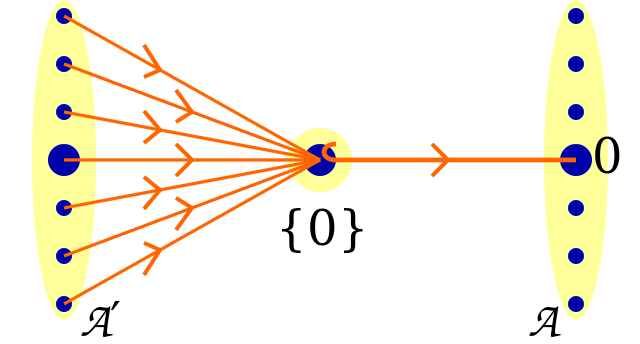
\includegraphics[scale=0.3]{img/01-obj.eps}
 %\captionsetup{labelformat=empty}
 \caption{零对象}
 \label{fig:zero-obj}
\end{figure}

平凡群中唯一的元素是什么名字不重要,它可以是$e$,可以是1(例如整数乘法群的平凡子群),可以是0(例如整数加群的平凡子群),可以是$I$(例如方阵乘法群中的单位矩阵),可以是(1)(置换群中的恒等置换),可以是$id$……在同构的意义下它们都是等价的。
\end{example}

\begin{example}
现在我们把难度增加一点,考虑全体集合的范畴$\pmb{Set}$,箭头是全函数。终止对象相对容易找到,就是只含有一个元素的集合(singleton)$\{ \bigstar \}$。仿照群的例子,对于任何集合$S$,我们让集合中所有的元素都映射到这个唯一的元素上去:$\forall x \in S, x \mapsto \bigstar$。显然这个箭头是唯一的。

\[
  S \longrightarrow \{ \bigstar \}
\]

但是问题来了,空集$\varnothing$怎样映射到$\{ \bigstar \}$上?事实上,空集\footnote{20世纪的伟大数学家,法国布尔巴基学派的成员安德烈$\cdot$韦伊说他发明了空集符号$\varnothing$,这是挪威语中的一个字母。}是集合范畴中的起始对象。对于任何集合$S$,我们都可以定义箭头

\[
  \varnothing \arrowto{f} S
\]

这一点比较难理解,请停下来仔细思考一下。可以从空集的$id$箭头出发思考这个问题,$\varnothing \arrowto{id_{\varnothing}} \varnothing$。根据范畴公理,$id$箭头是任何范畴中任何对象都有的。空集是到任何集合(包括它自己)都存在唯一箭头的对象。只不过这个箭头所表示的全函数没有任何参数。它不能写成$f(x): x \mapsto y$的形式。

回答刚才的问题,由于空集到任何集合都有唯一的箭头,所以空集到$\{ \bigstar \}$也有唯一的箭头。这样从任何集合(包括空集)都存在到$\{ \bigstar \}$的唯一箭头,因此$\{ \bigstar \}$的确是集合范畴中的终止对象。

为什么不能像群一样,让只含有一个元素的集合$\{ \bigstar \}$成为起始对象呢?原因是,从$\{ \bigstar \}$到任意集合$S$的箭头可能不唯一。考虑有若干元素的集合$S = \{x, y, z, ...\}$,我们可以定义箭头(全函数)$\{ \bigstar \} \arrowto{\vec{x}} S$,将唯一元素映射到$x$上,也可以定义箭头$\{ \bigstar \} \arrowto{\vec{y}} S$和$\{ \bigstar \} \arrowto{\vec{z}} S$,将其映射到其它元素上。

我们选择符号$\{ \bigstar \}$的用意是说,元素是什么不重要,只要它是只含有一个元素的集合(singleton set),在同构意义上就是等价的。

\label{sec:selection-arrow} \index{选择箭头}
从终止对象$\{ \bigstar \}$到某一集合$S$的箭头

\[
  \{ \bigstar \} \longrightarrow S
\]

也有着特定的含义。它表明我们可以从集合$S$中选出一个元素,例如上述的箭头$\vec{x}$,从集合中选出元素$x$。我们把这样的箭头叫做\textbf{选择箭头}。
\end{example}

\begin{example}
在最后一个例子中,我们来到编程领域。编程环境的类型系统本质上是集合范畴$\pmb{Set}$。一个集合相当于是一个数据类型。例如整形$Int$是所有整数的集合;布尔型是两个元素$\{True, False\}$组成的集合。既然集合范畴的终止对象是$\{ \bigstar \}$,那么什么数据类型是编程中的终止对象呢?由于终止对象在同构的意义下是唯一的,所以任何只含有一个值的数据类型都是编程中的终止对象。

为此,我们可以特别定义一个数据类型叫做“()”,它只含有一个元素,也叫做“()”。

\begin{lstlisting}
data  ()  =  ()
\end{lstlisting}

在同构的意义下$\{ \bigstar \} = \{()\}$,我们稍后会看到用“()”的好处。可以这样定义所有类型(集合)到这个终止对象的箭头(全函数):

\begin{lstlisting}
unit :: a -> ()
unit _ = ()
\end{lstlisting}

我们也可以自己定义终止对象——任何只有一个值的数据类型,在同构的意义上它和()是等价的\footnote{在其它编程环境,例如C++, Java,Scala中,可以定义“单子”(Single)对象,如果把强制类型转换作为箭头,则这也构成了终止对象。}。

\begin{lstlisting}
data Singleton = S

proj :: a -> Singleton
proj _ = S
\end{lstlisting}

看起来这像一个常函数,把任何值都映射到一个常数的值,但是并非所有常函数都指向终止对象,例如下面两个常函数:

\begin{lstlisting}
yes :: a -> Bool
yes _ = True

no :: a -> Bool
no _ = False
\end{lstlisting}

因为数据类型$Bool$包含两个元素,所以任何其他数据类型都有$yes, no$两个箭头指向$Bool$,这样就不满足终止对象箭头的唯一性要求。

在集合范畴中,起始对象是空集$\varnothing$,那么在编程中它对应着什么数据类型呢?既然数据类型本质上是集合,那么空集就相当于没有任何值的数据类型。在编程中,相当于我们声明了一个数据类型,但是却没有对它进行定义。

例如我们可以声明一个类型\texttt{Void},但是却没有为它定义任何值:

\begin{lstlisting}
data Void
\end{lstlisting}

这样\texttt{Void}就表示一个空集。但是起始对象必须有到所有其它对象的唯一箭头。这就要求我们必须定义从\texttt{Void}到所有其他类型的函数。

\begin{lstlisting}
absurd :: Void -> a
absurd _ = undefined
\end{lstlisting}

函数的具体实现并不重要,因为根本不存在一个实际的参数来调用这个函数。我们完全也可以这样定义:

\begin{lstlisting}
absurd :: Void -> a
absurd a = case a of {}
\end{lstlisting}

我们也可以自己定义起始对象,只要在同构的意义上是等价的就可以。方法就是只声明类型,不定义任何值。例如:

\begin{lstlisting}
data Empty

f :: Empty -> a
f _ = undefined

iso :: Void -> Empty
iso _ = undefined

iso' :: Empty -> Void
iso' _ = undefined
\end{lstlisting}

我们明确定义了$iso$和$iso'$,使得\texttt{Empty}和$\texttt{Void}$是同构的。并且容易验证\texttt{iso . iso' = id}。

集合范畴的例子中,我们说从终止对象到任何集合的箭头叫做选择箭头,它在编程中意味着什么呢?集合对应着类型,它表示我们可以从任何类型中选出特定的值。例如下面的函数从$Int$中分别选出0和1:

\begin{lstlisting}
zero :: () -> Int
zero () = 0

one :: () -> Int
one () = 1
\end{lstlisting}

现在我们看到用“()”的好处了,调用的时候,就像传入0个参数的函数那样:$zero\ ()$返回0,$one\ ()$返回1。
\end{example}

\begin{Exercise}
\Question{在本节的例子中,我们说在一个偏序集中,如果存在最小值(或最大值),则最小值(或最大值)就是起始对象(或终止对象)。考虑全体偏序集构成的范畴$\pmb{Poset}$,如果存在起始对象,它是什么?如果存在终止对象,它是什么?}
\Question{皮亚诺范畴$\pmb{Pno}$(参见本章第一节的习题2)中,什么样的对象$(A, f, z)$是起始对象?终止对象是什么?}
\end{Exercise}

\subsection{幂}
\index{幂} \index{exponential}

起始对象和终止对象,相当于0和1,积和余积相当于$\times$和$+$,如果再有了指数(幂),我们就可以在范畴这个抽象层面中拥有和基本算术运算,甚至和多项式“同构”的强大工具。

观察一个定义在自然数上二元函数$f(x, y) = z$,例如$f(x, y) = x^2 + 2y + 1$。其类型为$f: N \times N \to N$。我们会自然联想到,可以把这个类型写成:

\[
f : N^2 \to N
\]

对于函数$f$,我们能否把$N^2$看成一个对象,而不是两个参数呢?也就是说,看成$f\ (x, y)$,而不是$f(x, y)$。如果把参数看成一个“洞”,则前者是$f\ \bullet$,然后把一个对$(x, y)$填入洞中;而后者是$f(\bullet, \bullet)$,然后分别把$x, y$填入到两个洞中。另一方面,在第二章我们介绍了克里化,可以把$f$看成$f: N \to (N \to N)$,也就是传入$x$后,$f\ x$会返回另一个函数,这个新函数把一个自然数映射到另一个自然数。但使用克里化,我们反而得不到幂的概念了。峰回路转,如果我们把克里化后返回的东西,也就是$N \to N$看成一个事物,比方叫做“函数对象”会怎样呢?$N$是一个无穷集,想起来比较困难。我们后退一步,构造一个简单点的例子——只有两个元素的有限集$Bool$——来分析一下。

\begin{example}
存在无穷多个从$Bool$到$Int$的函数(箭头)组成的集合$\{Bool \arrowto{f} Int\}$,我们从这个集合中挑选一个元素,也就是一个例子函数来看看:

\[
\begin{array}{l}
ord : Bool \to Int \\
ord\ False = 0 \\
ord\ True = 1 \\
\end{array}
\]

它的结果是一对整数$(0, 1)$,这是一个代表,我们可以把所有上述箭头集合中的元素写成这样的形式:

\[
\begin{array}{l}
f : Bool \to Int \\
f\ False = ... \\
f\ True = ... \\
\end{array}
\]

不管$f$怎样千变万化,结果总是一对整数$(a, b)$。我们可以说箭头$f$的集合,同构于一对整数$(a, b)$的集合,即:

\[
\begin{array}{rcl}
\{Bool \arrowto{f} Int\} & = & \{(a = f\ False, b = f\ True)\} \\
  & = & Int \times Int \\
  & = & Int^2 = Int^{Bool}
\end{array}
\]

这告诉我们,箭头的集合,也就是箭头的类型\footnote{严格来说,我们应该去掉上面箭头两侧的大括号,增加大括号是为了容易理解}:$Bool \to Int$,相当于一个幂$Int^{Bool}$。也就是说$Bool \to Int = Int^{Bool}$。为什么在上面的推理中,我们可以用$Bool$替换$2$,从而把$Int^2$变成$Int^{Bool}$呢?原因是同构,上述的等号的真正含义是同构,所以严格来说,应该用“$\cong$”符号,而不是“=”。$Int^2$,是两个整数积的自然记法,也就是一对$Int$值的集合。一对$Int$值的集合可以看成是从一个名叫\textbf{2}的,拥有2个元素的索引集合$\{0, 1\}$到$Int$的映射。

\[
\{0, 1\} \arrowto{f} Int = \{(f(0), f(1))\} = Int^2
\]

而索引集合$\mathbf{2} = \{0, 1\}$正是$Bool$的同构(例如在$ord$函数下)。
\end{example}

\begin{example}
再举一个例子,考虑所有从字符$Char$到布尔值$Bool$的函数(箭头)集合$Char \to Bool$。这个集合里有很多函数,例如$isDigit(c)$可以判断传入的字符是否是数字。它可以实现为:

\lstset{frame=none}
\begin{lstlisting}[style=Haskell]
isDigit : Char -> Bool
...
isDigit '0' = True
isDigit '1' = True
...
isDigit '9' = True
isDigit 'a' = False
isDigit 'b' = False
...
\end{lstlisting}

虽然这个实现比较的笨拙,但是它反映了一个事实:如果$Char$中有256个不同的字符(例如英语ASCII码),则函数$isDigit$的结果本质上和一个256元组(False, ..., True, True, ... True, False, ...)同构。这个元组中对应数字字符的位置是True,其余是False。在$Char \to Bool$中的众多函数中,$isUpper$,$isLower$,$isWhitespace$等等分别对应一个特定的元组。例如$isUpper$对应的元组中,大写字符所在的位置上为True,其余为False。这样尽管有无穷多种方式来定义一个从$Char$到$Bool$的函数,但从结果上看,本质上只有$2^{256}$个不同的函数。也就是说$Char \to Bool$和256元组的布尔值集合$Bool^{Char}$同构。
\end{example}

现在我们把例子中的集合推进到无限集。在这一节的开头,我们说克里化后的函数$f: N \to (N \to N)$,是从自然数$N$到“函数对象”的函数。我们把函数对象记为$(\Rightarrow)$,则$f$的类型为$N \arrowto{f} (\Rightarrow)$。也就是从索引集$\{0, 1, ...\}$到$(\Rightarrow)$的映射,它是一个无穷长元组的集合,元组的每个值都是一个函数对象。记为$(\Rightarrow)^N$。

\index{apply}
一般来说,我们把函数的集合$f : B \to C$记为$C^B$。从这个集合中取出一个函数$f \in C^B$,然后在从集合$B$中取出一个值$b \in B$,我们可以用一个名叫$apply$的函数将$f$应用到$b$上,从而得到一个$C$中的值$c = f(b)$。即\footnote{有些文献,例如\cite{PeterSmith2018}第111-112页, \cite{Wiki-Exponentials}使用$eval$,也就是求值(evaluation)作为名称,这里采用和\cite{Bird97}(第72页)一致的命名。这样和Lisp中的命名传统一致。}:

\[
apply(f, b) = f(b)
\]

聪明的读者可能会问:符号$A$哪里去了?因为$A$还有别的用处。我们还要把克里化考虑进来。对于二元函数$g: A \times B \to C$,传入一个$A$中的值$a$后,就得到了一个克里化的函数$g(a, \bullet) : B \to C$。它是一个函数对象,属于$C^B$。这样,对于任何二元函数$A \times B \arrowto{g} C$,都存在唯一的一元函数$A \arrowto{\lambda g} C^B$,将$a \in A$送入$g(a, \bullet) : B \to C$中。我们称$\lambda g$为$g$的幂转换(exponential transpose)\footnote{有的文献中用$\bar{g}$来表示,根据第二章中对$\lambda$的介绍,以及关于丘奇出版商的小插曲,我认为用$\lambda g$更为传神,它表示$a \mapsto \lambda \bullet \cdot g(a, \bullet)$。}。并且,有这样的关系:


\[
apply(\lambda g(a), b) = g(a, b)
\]

也就是说,$apply$把一个类型为$C^B$的函数对象$\lambda g(a)$与类型为$B$的参数$b$组合在一起,最终得到类型为$C$的结果$c$。所以箭头$apply$的类型为:

\[
C^B \times B \arrowto{apply} C
\]

\index{幂对象(Exponentials或Exponential object)}
现在,我们终于可以给出完整的幂对象(Exponentials或Exponential object)定义了。

\begin{definition}
如果范畴$\pmb{C}$中存在终止对象和积,则一个\textbf{幂对象}是一对对象和箭头

\[
(C^B, apply)
\]

它们满足对于任何的对象$A$和箭头$A \times B \arrowto{g} C$,都存在唯一的转换箭头

\[
 A \arrowto{\lambda g} C^B
\]

使得下面的范畴图可交换

\begin{center}
\begin{tikzpicture}
  \matrix (m) [matrix of math nodes,
               row sep=3em, column sep=5em, minimum width=2em]{
     A & A \times B & \\
     C^B & C^B \times B & C \\};
  \path[-stealth]
    (m-1-1) edge node [left] {$\lambda g$} (m-2-1)
    (m-1-2) edge node [left] {$\lambda g \times id_B$} (m-2-2)
    (m-1-2) edge node [above] {$g$} (m-2-3)
    (m-2-2) edge node [below] {$apply$} (m-2-3);
\end{tikzpicture}
\end{center}

即:

\[
  apply \circ (\lambda g \times id_B) = g
\]

\end{definition}

\index{克里化}
第二章中我们没有给出克里化的完整定义,现在利用幂对象,我们可以给出$curry$的定义了:

\[
\begin{array}{l}
curry : (A \times B \to C) \to A \to (C^B) \\
curry\ g = \lambda g
\end{array}
\]

因此,$curry\ g$就是$g$的幂转换。把这一关系代入上面的范畴图,我们有:

\[
  apply \circ (curry\ g \times id) = g
\]

换言之,我们就得到了这样的泛性性质:

\[
  f = curry\ g \quad \equiv \quad apply \circ (f \times id) = g
\]

并且我们还能说明为什么幂转换箭头是唯一的,假设还存在另外的箭头$A \arrowto{h} C^B$,使得$apply \circ (h \times id) = g$,根据上述泛性性质,我们立刻得到$h = curry\ g$。

我们还可以从范畴的角度来理解幂对象,在范畴$\pmb{C}$中,如果固定对象$B, C$,我们可以构造一个名叫$\pmb{Exp}$的范畴,这个范畴中的对象是$A \times B \to C$这样的箭头,范畴中的箭头是这样定义的:

\begin{center}
\begin{tikzpicture}
  \matrix (m) [matrix of math nodes,
               row sep=3em, column sep=5em, minimum width=2em]{
     A & A \times B \arrowto{h} C \\
     D & D \times B \arrowto{k} C \\};
  \path[-stealth]
    (m-1-1) edge node [left] {$f$} (m-2-1)
    (m-1-2) edge node [left] {$j$} (m-2-2);
\end{tikzpicture}
\end{center}

如果在$\pmb{C}$中存在$A \arrowto{f} D$的箭头,则$\pmb{Exp}$中的箭头为$h \arrowto{j} k$。当且仅当把上面范畴图中右侧的$C$合并时,箭头之间可交换:

\begin{center}
\begin{tikzpicture}
  \matrix (m) [matrix of math nodes,
               row sep=3em, column sep=5em, minimum width=2em]{
     A & A \times B & \\
     D & D \times B & C \\};
  \path[-stealth]
    (m-1-1) edge node [left] {$f$} (m-2-1)
    (m-1-2) edge node [left] {$f \times id_B$} (m-2-2)
    (m-1-2) edge node [above] {$h$} (m-2-3)
    (m-2-2) edge node [below] {$k$} (m-2-3);
\end{tikzpicture}
\end{center}

即:$k \circ (f \times id_B) = h$。在这个范畴$\pmb{Exp}$中,存在一个终止对象,它恰好是$C^B \times B \arrowto{apply} C$。我们现在来验证一下,根据幂对象的定义,从任何其它对象$A \times B \arrowto{g} C$,都有到$apply$的箭头$\lambda g = curry\ g$。另外根据终止对象的性质,从终止对象到自己的箭头一定是$id$,所以我们有\textbf{反射律}:

\[
curry\ apply = id
\]

\begin{Exercise}
\Question{验证$\pmb{Exp}$的确是一个范畴,指出$id$箭头和箭头的组合。}
\Question{反射律$curray\ apply = id$中,$id$的下标是什么?请用另一种方法证明它。}
\Question{我们称下面的等式
\[
(curry\ f) \circ g = curry(f \circ (g \times id))
\]
为克里化的融合律。请画出它的范畴图并证明它。}
\end{Exercise}

\subsection{笛卡尔闭和对象算术}

有了起始对象0,终止对象1,余积代表的加法,积代表的乘法,再加上幂对象代表的指数幂,我们终于拥有了在范畴上进行运算甚至构造抽象多项式的能力。但是且慢,让我们停下来看一下这样能跑多远。正如第三章开头我们讲到的,必须时刻关注一个问题:“某一种抽象的适用范围有多大?什么情况下这一抽象会失效?”

\index{笛卡尔闭}
并非所有的范畴都有起始或终止对象,也并非所有的范畴都有幂对象。如果一个范畴存在有限积、对于任何对象$A$和$B$都存在幂$A^B$,我们称这样的范畴为\textbf{笛卡尔闭}的(Cartesian closed)。一个笛卡尔闭范畴必须包含:

\begin{enumerate}
\item 一个终止对象(1);
\item 任何一对对象都有积($\times$);
\item 任何一对对象都有幂($A^B$)
\end{enumerate}

我们既可以把终止对象1,想象成一个对象的零次幂:$A^0 = 1$,也可以把它想象成零个对象的积。非常幸运的是,编程时我们所在的范畴——集合和全函数组成的范畴是笛卡尔闭的。一个笛卡尔闭范畴可以作为简单类型$\lambda$-演算(simply typed lambda calculus)的数学模型(见第二章),从而成为所有带有类型的编程语言的基础(\cite{Milewski2018}第148页)。

\index{双笛卡尔闭(Bicartesian closed)}
如果一个笛卡尔闭的范畴还同时支持终止对象的对偶——起始对象,和积的对偶——余积。并且支持积和余积的分配律,我们称其为\textbf{双笛卡尔闭}范畴(Bicartesian closed):

\begin{enumerate}
  \setcounter{enumi}{4}
  \item 一个起始对象(0);
  \item 任何一对对象都有余积($+$);
  \item 积可以从左右两侧分配到余积上:
  \[
  \begin{array}{l}
  A \times (B + C) = A \times B + A \times C \\
  (B + C) \times A = B \times A + C \times A
  \end{array}
  \]
\end{enumerate}

\index{对象算术}
现在我们可以看看基本算术运算在一个笛卡尔闭的范畴上,特别是编程中都意味着什么了。这一理论称为对象算术理论(Equational theory)。

\subsubsection{0次幂}

\[
  A^0 = 1
\]

0代表了起始对象,1代表了终止对象,$A$的0次幂可以解读为类型为$0 \to A$的所有箭头的集合。但既然0是起始对象,所以它到任何对象只有唯一的箭头。因此集合$\{ 0 \to A \}$仅仅含有一个元素(singleton),而仅有一个元素的集合$\{ \bigstar \}$恰巧是(集合范畴的)终止对象1。下面的推导中等号应理解为同构。

\[
\begin{array}{rcll}
A^0 & = & \{ 0 \to A \} & \text{幂对象的定义} \\
    & = & \{ \bigstar \} & \text{起始对象到任何对象的箭头唯一} \\
    & = & 1 & \{ \bigstar \}\text{是终止对象} \\
\end{array}
\]

这样,算术中的任何数的0次幂等于1在范畴中也得到了解读。

\subsubsection{1的幂}

\[
  1^A = 1
\]

1代表了终止对象,所以幂对象$1^A$表示所有从$A$出发,到终止对象的箭头的集合$\{ A \to 1 \}$。根据终止对象的定义,任何对象到终止对象只有唯一的箭头,所以这个箭头集合仅仅含有一个元素,而仅有一个元素的集合同构于$\{ \bigstar \}$。它恰好又是(集合范畴中的)终止对象。

\[
\begin{array}{rcll}
1^A & = & \{ A \to 1 \} & \text{幂对象的定义} \\
    & = & \{ \bigstar \} & \text{任何对象到终止对象的箭头唯一} \\
    & = & 1 & \{ \bigstar \}\text{是终止对象} \\
\end{array}
\]

\subsubsection{1次幂}

\[
  A^1 = A
\]

这恰好是前面介绍过的“\hyperref[sec:selection-arrow]{选择箭头}”。1是终止对象,所以幂$A^1$表示了从终止对象到$A$的箭头集合$\{ 1 \to A\}$。如果$A$是一个集合,我们可以针对集合中的任何元素$a \in A$构造一个从终止对象1到$a$的一个函数:

\[
  f_a : 1 \to a
\]

这种选择函数,能从集合$A$中选出一个元素$a$。所有从1到$A$中元素的选择函数的集合为$\{f_a : 1 \mapsto a | a \in A\}$,它恰好就是集合$1 \to A$。另一方面,集合$\{ f_a \}$是和$A = \{a\}$一一对应的,也就是说它们是同构的。

\[
\begin{array}{rcll}
A^1 & = & \{ 1 \to A \} & \text{幂对象的定义} \\
    & = & \{ f_a : 1 \mapsto a | a \in A \} & \text{从1到$A$中元素的映射的集合} \\
    & = & \{ a | a \in A \} = A & \text{一一映射同构} \\
\end{array}
\]

\subsubsection{幂的和}

\[
  A^{B + C} = A^B \times A^C
\]

幂对象$A^{B + C}$表示从余积$B + C$到$A$的箭头的集合$\{B + C \to A\}$。我们借助$\mathbf{Either}\ B\ C$来帮助我们思考\footnote{也可以用标记(tag)来推理:
\[
\begin{array}{l}
f : B + C \to A \\
f (b, 0) = ... \\
f (c, 1) = ...
\end{array}
\]
},当我们实现任何$\mathbf{Either}\ B\ C \to A$函数时,都可以写成这样的形式:

\[
\begin{array}{l}
f : \mathbf{Either}\ B\ C \to A \\
f\ left\ b = ... \\
f\ right\ c = ... \\
\end{array}
\]

也就是说,任何这样的函数,都可以看作一对映射$(b \mapsto a_1, c \mapsto a_2)$,而$\{(b \mapsto a_1, c \mapsto a_2)\}$恰好是$B \to A$和$C \to A$的积。因此$\{B + C \to A\} = \{B \to A\} \times \{C \to A\}$。另一方面,根据$\{B \to A\}$可以表示为幂对象$A^B$,同样$\{C \to A\}$可以表示为$A^C$。这样就解读了幂的和:

\[
\begin{array}{rcll}
A^{B + C} & = & \{ B + C \to A \} & \text{幂对象的定义} \\
    & = & \{ (b \mapsto a_1,  c \mapsto a_2) | a_1, a_2 \in A, b \in B, c \in C\} & \text{$B$和$C$到$A$的箭头对} \\
    & = & \{ B \to A \} \times \{ C \to A \} & \text{笛卡尔积} \\
    & = & A^B \times A^C & \text{幂对象} \\
\end{array}
\]

\subsubsection{幂的幂}

\[
  (A^B)^C = A^{B \times C}
\]

先看右侧,幂对象$A^{B \times C}$实际就是二元函数$B \times C \arrowto{g} A$的集合。交换积的次序$C \times B \arrowto{g \circ swap} A$,显然是一个自然同构(参见自然同构一节的$swap$自然变换)。如果克里化,就是$\{curry(g \circ swap)\} = \{C \to A^B\}$,再一次用幂对象表示就是$(A^B)^C$。

\[
\begin{array}{rcll}
A^{B \times C} & = & \{B \times C \arrowto{g} A \}  & \text{幂对象的定义} \\
    & = & \{ C \times B \arrowto{g \circ swap} A \} & \text{自然同构} \\
    & = & \{ C \arrowto{curry(g \circ swap)} A^B \} & \text{克里化后仍然同构} \\
    & = & (A^B)^C & \text{幂对象} \\
\end{array}
\]

\subsubsection{积的幂}

\[
  (A \times B)^C = A^C \times B^C
\]

幂对象$(A \times B)^C$是箭头$C \to A \times B$的集合,它可以认为是返回一对值的函数集合$\{ c \mapsto (a, b)\}$,其中$c \in C, a \in A, b \in B$。它显然同构于$\{(c \mapsto a, c \mapsto b)\}$,而这恰恰是箭头$C \to A$和$C \to B$的积。最后再分别将$C \to A$和$C \to B$表示为幂对象就得到了幂的积。

\[
\begin{array}{rcll}
(A \times B)^C & = & \{C \to A \times B \}  & \text{幂对象的定义} \\
    & = & \{ c \mapsto (a, b) | a \in A, b \in B, c \in C\} & \text{箭头的集合} \\
    & = & \{ (c \mapsto a, c \mapsto b) \} & \text{箭头对} \\
    & = & \{C \to A\} \times \{C \to B\} & \text{笛卡尔积} \\
    & = & A^C \times B^C & \text{幂对象} \\
\end{array}
\]

\subsection{多项式函子}
\label{sec:polynomial-functors}
\index{多项式函子}

以上介绍的在笛卡尔闭范畴上的算术主要是针对对象的。如果我们把函子考虑进来,会怎样呢?由于函子既作用于对象,也作用于箭头,这样就产生了多项式函子的概念。多项式函子是使用常函子(参见\hyperref[sec:functor:examples]{函子的例子中的“黑洞”函子})、积函子和余积函子递归构造的。

\begin{itemize}
  \item 恒等函子$id$和常函子$\mathbf{K}_A$是多项式函子;
  \item 若函子$\mathbf{F}$和$\mathbf{G}$是多项式函子,则它们的组合$\mathbf{FG}$,和$\mathbf{F} + \mathbf{G}$与积$\mathbf{F} \times \mathbf{G}$也是多项式函子。其中和与积定义如下:
  \[
    \begin{array}{l}
    (\mathbf{F} + \mathbf{G}) h = \mathbf{F} h + \mathbf{G} h \\
    (\mathbf{F} \times \mathbf{G}) h = \mathbf{F} h \times \mathbf{G} h \\
    \end{array}
  \]
\end{itemize}

举一个例子,若函子$\mathbf{F}$对于对象和箭头的行为是:

\[
\begin{cases}
\text{对象:} & \mathbf{F} X = A + X \times A \\
\text{箭头:} & \mathbf{F} h = id_A + h \times id_A
\end{cases}
\]

其中$A$是某个固定的对象。则函子$\mathbf{F}$是一个多项式函子。这是因为它可以表达为多项式:

\[
\mathbf{F} = \mathbf{K}_A + (id \times \mathbf{K}_A)
\]

\subsection{F-代数}

为了构造复杂的带有递归结构的代数数据类型,我们还需要最后一块砖石。这就是F-代数(F-algebras)。观察抽象代数中的概念,如幺半群、群、环、域,它们不仅仅是抽象的对象,而且带有结构。正是这些结构之间的关系,使得它们区别于过去那些具体的对象,例如数、点、线、面。如果关系和结构研究清楚了,不仅仅是数、点、线、面,所有具有同样关系和结构的对象(用希尔伯特的比喻,连同桌子、椅子、啤酒杯)就都尽在掌握了。

\begin{example}
我们从比较简单的幺半群作为开始的例子,一步一步导出F-代数的概念。一个幺半群是一个集合$M$,并且在集合上定义了可结合的二元运算和单位元。

如果用$\oplus$表示二元运算,$1_M$表示单位元,则幺半群的两条公理可以描述如下:

\[
\begin{cases}
\text{结合性公理:} & (x \oplus y) \oplus z = x \oplus (y \oplus z), \forall x, y, z \in M \\
\text{单位元公理:} & x \oplus 1_M = 1_M \oplus x = x, \forall x \in M \\
\end{cases}
\]

第一步,我们将二元运算$\oplus$表示为函数,将$1_M$表示为选择函数,定义:

\[
\begin{cases}
m (x, y) = x \oplus y \\
e () = 1_M
\end{cases}
\]

这两种箭头的类型分别为:

\[
\left \{
\begin{array}{lll}
 & \text{类型} & \text{幂对象} \\
\text{二元运算:} & M \times M \to M & M^{M \times M}\\
\text{选择运算:} & 1 \to M & M^1 \\
\end{array}
\right .
\]

第一种箭头是说,两个幺半群的元素进行二元运算,其结果仍是这个幺半群中的元素(二元运算是封闭的);第二种箭头是“选择函数”,1是终止对象\footnote{我们特意用“()”表示终止对象,在同构的意义下$1 = \{ \bigstar \} = \{ () \}$。这样的好处是,$e()$看起来像是个无参数的函数调用,实际接受了终止对象中的唯一元素()作为参数。}。

现在我们就可以用函数$m$和$e$来替换幺半群公理了:

\[
\begin{cases}
\text{结合性公理:} & m(m(x, y), z) = m(x, m(y, z)), \forall x, y, z \in M \\
\text{单位元公理:} & m(x, e()) = m(e(), x) = x, \forall x \in M \\
\end{cases}
\]

第二步,把所有的$x, y, z$等具体的元素和对象$M$都去掉。这样就得到了纯用函数(箭头)表示的幺半群公理:

\[
\begin{cases}
\text{结合性公理:} & m \circ (m, id) = m \circ (id, m) \\
\text{单位元公理:} & m \circ (id, e) = m \circ (e, id) = id \\
\end{cases}
\]

这两条公理意味着下面的两个范畴图中的箭头可交换:

\begin{figure}[htbp]
\centering
\subcaptionbox{结合性公理}{\subimport{img/}{monoid-assoc.tex}}
\quad
\subcaptionbox{单位元公理}{\subimport{img/}{monoid-e.tex}}
\caption{幺半群公理对应的范畴图}
\end{figure}

现在可以说,任何幺半群都可以用一个三元组$(M, m, e)$来表示了。其中$M$是集合,$m$是二元运算函数,$e$是单位元选择函数。

第三步,$(M, m, e)$不仅规定了幺半群的集合,还规定了在此集合上的二元运算和单位元,因此整个幺半群的代数结构就都确定了。组成幺半群的所有箭头,也就是代表所有可能的$m$和$e$的箭头集合,是两种幂对象的积

\[
M^{M \times M} \times M^1 = M^{M \times M + 1}
\]

我们再把右侧从幂对象写回箭头的形式,这样集合$M$上定义的幺半群代数运算一定是下面的形式:

\[
\begin{array}{rcll}
\alpha : 1 + M \times M & \longrightarrow & M & \text{和(余积)}\\
1 & \longmapsto & 1 & \text{单位元}  \\
(x, y) & \longmapsto & x \oplus y & \text{二元运算}
\end{array}
\]

通过余积用和来表示这种关系就是$\alpha = e + m$,用多项式函子来表示就是$\mathbf{F} M = 1 + M \times M$

总结一下,对于幺半群这个例子,幺半群上的代数结构由三部分组成:

\begin{enumerate}
  \item 对象$M$,就是用于携带幺半群上代数结构的集合,叫做\textbf{携带对象}(carrier object);
  \item 函子$\mathbf{F}$,定义了幺半群上的代数运算。是一个多项式函子$\mathbf{F} M = 1 + M \times M$;
  \item 箭头$\mathbf{F} M \arrowto{\alpha} M$,它是单位元箭头$e$和二元运算箭头$m$的和(余积),$\alpha = e + m$。
\end{enumerate}

我们称这样定义了一个幺半群的$F$-代数$(M, \alpha)$。

例如在编程中,可以这样定义一个F-代数箭头的类型:

\begin{lstlisting}
type Algebra f a = f a -> a
\end{lstlisting}

这本质上是给箭头$\mathbf{F}A \to A$起了一个别名(alias),名叫\texttt{Algebra} $\mathbf{F}, A$。对于幺半群,还需要定义一个函子\footnote{
Haskell中有一个对幺半群的标准定义(见本章附录)。但这是一个幺半群代数结构的定义,而不是幺半群函子。}:

\begin{lstlisting}
data MonoidF a = MEmptyF | MAppendF a a
\end{lstlisting}

当\texttt{a}是字符串时,我们可以这样定义一个F-代数\texttt{(String, evals)}的箭头实现:

\begin{lstlisting}
evals :: Algebra MonoidF String
evals MEmpty = e ()
evals (MAppendF s1 s2) = m s1 s2

e :: () -> String
e () = ""

m :: String -> String -> String
m = (++)
\end{lstlisting}

当然,也可将\texttt{e}和\texttt{m}内嵌到\texttt{evals}中简化实现为:

\begin{lstlisting}
evals :: Algebra MonoidF String
evals MEmpty = ""
evals (MAppendF s1 s2) = s1 ++ s2
\end{lstlisting}

\texttt{evals}是箭头$\alpha : \mathbf{F}A \to A$的一种实现,其中$\mathbf{F}$为\texttt{MonoidF},$A$为\texttt{String}。当然还可以有别的实现,只要它能够满足幺半群的单位元公理和结合性公理。
\end{example}

\begin{example}
在幺半群之上,增加一条可逆性公理,就得到了群。我们仍然分步骤引出群的F-代数。首先列出群元素集合$G$上的三条公理,我们用$1_G$表示单位元,点号表示二元运算,$()^{-1}$表示求逆元:

\[
\begin{cases}
\text{结合性公理:} & (x \cdot y) \cdot z = x \cdot (y \cdot z), \forall x, y, z \in G \\
\text{单位元公理:} & x \cdot 1_G = 1_G \cdot x = x, \forall x \in G \\
\text{可逆性公理:} & x \cdot x^{-1} = x^{-1} \cdot x = 1_G, \forall x \in G
\end{cases}
\]

第一步,将二元运算,求单位元、求逆元都表示为函数。定义:

\[
\begin{cases}
m (x, y) = x \cdot y \\
e () = 1_G \\
i (x) = x^{-1}
\end{cases}
\]

这三种函数的类型和幂对象分别为:

\[
  \left \{
    \begin{array}{lll}
      \text{二元运算:} & G \times G \to G & G^{G \times G}\\
      \text{选择运算:} & 1 \to G & G^1 \\
      \text{求逆运算:} & G \times G & G^G \\
    \end{array}
  \right . \\
\]

前两个箭头和幺半群一样,第三个箭头是说群元素的逆元仍是群中的元素。现在就可以用$e, m ,i$替换群公理中的$1_G$,点号和逆元符号了。

\[
\begin{cases}
\text{结合性公理:} & m(m(x, y), z) = m(x, m(y, z)), \forall x, y, z \in G \\
\text{单位元公理:} & m(x, e()) = m(e(), x) = x, \forall x \in G \\
\text{可逆性公理:} & m(x, i(x)) = m(i(x), x) = e(), \forall x \in G \\
\end{cases}
\]

第二步,把所有的具体元素$x, y, z$和群元素集合$G$去掉。得到纯用箭头表示的群公理:

\[
\begin{cases}
\text{结合性公理:} & m \circ (m, id) = m \circ (id, m) \\
\text{单位元公理:} & m \circ (id, e) = m \circ (e, id) = id \\
\text{可逆性公理:} & m \circ (id, i) = m \circ (i, id) = e \\
\end{cases}
\]

这样,任何群都可以用一个四元组$(G, m, e, i)$表示。

第三步,利用余积求$m, e, i$的和$\alpha = e + m + i$,通过多项式函子$\mathbf{F} A = 1 + A + A \times A$,并令$A = G$,描述群$G$上的代数运算。

\[
\begin{array}{rcll}
\alpha : 1 + A + A \times A & \longrightarrow & A & \text{和(余积)}\\
1 & \longmapsto & 1 & \text{单位元}  \\
x & \longmapsto & x^{-1} & \text{逆元} \\
(x, y) & \longmapsto & x \cdot y & \text{二元运算} \\
\end{array}
\]

所以,群上的代数结构由三部分组成:

\begin{enumerate}
  \item 携带对象$G$,用于携带群上代数结构的集合;
  \item 多项式函子$\mathbf{F} A = 1 + A + A \times A$,定义了群上的代数运算;
  \item 箭头$\mathbf{F} A \arrowto{\alpha = e + m + i} A$,它是单位元箭头$e$、二元运算箭头$m$、逆元箭头$i$的和。
\end{enumerate}

我们称这样定义了一个群上的F-代数$(G, \alpha)$。
\end{example}

\index{F-代数} \index{F-余代数}
现在我们可以给出F-代数的定义了。在范畴论中,许多概念是对偶的,成对出现的。这就像是买一送一,我们定义了F-代数,就同时得到了F-余代数(F-coalgebra)\footnote{也译作上代数和共代数。}。关于F-余代数,我们暂时只给出定义。稍后将在第6章介绍无穷的概念时,再给出相应的例子。

\begin{definition}
如果$\pmb{C}$是一个范畴,$\pmb{C} \arrowto{\mathbf{F}} \pmb{C}$是范畴$\pmb{C}$上的一个自函子。对于范畴中的对象$A$和态射$\alpha$:

\[
  \mathbf{F} A \arrowto{\alpha} A
  \quad \quad \quad
  A \arrowto{\alpha} \mathbf{F} A
\]

构成一对元组$(A, \alpha)$叫做

\begin{center}
  F-代数 \quad \quad \quad F-余代数
\end{center}

其中$A$,叫做携带对象。

\end{definition}

我们可以把

\begin{center}
  F-代数$(A, \alpha)$ \quad \quad \quad F-余代数$(A, \alpha)$
\end{center}

本身看成对象。在上下文清楚的情况下,我们通常用二元组$(A, \alpha)$表示对象。
两个对象间的箭头定义如下:

\begin{definition}
F-态射是F-代数或F-余代数对象间的箭头:

\[
  (A, \alpha) \longrightarrow (B, \beta)
\]

如果携带对象间的箭头$A \arrowto{f} B$,使得下面的范畴图可交换:

\begin{center}
\begin{tikzpicture}
  \matrix (m) [matrix of math nodes,
               row sep=3em, column sep=3em, minimum width=2em]{
    \mathbf{F} A  & A &  & A & \mathbf{F} A \\
    \mathbf{F} B  & B &  & B & \mathbf{F} B \\};
  \path[-stealth]
    % left
    (m-1-1) edge node [above] {$\alpha$} (m-1-2)
    (m-1-1) edge node [left] {$\mathbf{F}(f)$} (m-2-1)
    (m-1-2) edge node [right] {$f$}   (m-2-2)
    (m-2-1) edge node [below] {$\beta$} (m-2-2)
    % right
    (m-1-4) edge node [above] {$\alpha$} (m-1-5)
    (m-1-4) edge node [left] {$f$} (m-2-4)
    (m-1-5) edge node [right] {$\mathbf{F}(f)$}   (m-2-5)
    (m-2-4) edge node [below] {$\beta$} (m-2-5);
\end{tikzpicture}
\end{center}

即:

\[
  f \circ \alpha = \beta \circ \mathbf{F}(f)
  \quad \quad \quad
  \beta \circ f = \mathbf{F}(f) \circ \alpha
\]
\end{definition}

F-代数和F-态射,F-余代数和F-态射分别构成了

\begin{center}
  F-代数范畴$\pmb{Alg}(\mathbf{F})$ \quad \quad \quad
  F-余代数范畴$\pmb{CoAlg}(\mathbf{F})$
\end{center}

\begin{Exercise}
\Question{画出群的可逆性公理的范畴图。}
\Question{$p$是一个素数,使用群的F-代数,为整数模$p$乘法群(可以参考上一章)定义一个$\alpha$箭头。}
\Question{参考上一章环的定义,定义环的F-代数。}
\Question{F-代数范畴上的$id$箭头是什么?箭头组合是什么?}
\end{Exercise}

\subsubsection{递归和不动点}

在第一章中,我们介绍了自然数和皮亚诺公理。并且介绍了和自然数同构的事物。实际上,我们可以把所有类似自然数的东西都用F-代数描述。

假设有一个集合$A$,具有自然数的代数结构。例如第一章中介绍过的斐波那契数列,其中$A$是数对$(Int, Int)$。起始对象是$(1, 1)$,后继函数是$h(m, n) = (n, m + n)$。

为了用F-代数描述这一\textbf{类}代数结构,我们需要三样东西:函子,携带对象和$\alpha$箭头。根据皮亚诺公理,自然数的函子应当这样定义:

\lstset{frame=none}
\begin{lstlisting}
data NatF A = ZeroF | SuccF A
\end{lstlisting}

这个函子是一个多项式函子$\mathbf{NatF} A = 1 + A$。现在我们提出一个问题。如果令$A’ = \mathbf{NatF} A$,将其代入$\mathbf{NatF}$函子,那么$\mathbf{NatF} A'$是什么?应该是两重函子$\mathbf{NatF}(\mathbf{NatF} A)$。我们还可以重复这一过程得到三重的$\mathbf{NatF}(\mathbf{NatF}(\mathbf{NatF} A))$。我们可以重复无穷多次,现在我们给重复无穷多次后产生类型$\mathbf{NatF}(\mathbf{NatF}(...))$起名为$\mathbf{Nat}$,即:

\[
\begin{array}{rcll}
\texttt{data}\ \mathbf{Nat} & = & \mathbf{NatF}(\mathbf{NatF}(...)) & \text{无穷重} \\
         & = & ZeroF\ |\ SuccF\ (SuccF (...)) & \text{无穷重}SuccF \\
         & = & ZeroF\ |\ SuccF\ \mathbf{Nat} & \text{无穷重}SuccF\text{的类型是}\mathbf{Nat} \\
         & = & Zero\ |\ Succ\ \mathbf{Nat} & \text{重命名}
\end{array}
\]

这恰恰是我们在第一章定义的自然数类型。我们把\texttt{Nat}和\texttt{Nat A}并列写在一起:

\begin{lstlisting}
data Nat = Zero | Succ Nat

data NatF A = ZeroF | SuccF A
\end{lstlisting}

这是函子层面的递归,在第二章中,我们曾经遇到过类似的概念。将自函子应用到自身无穷次产生了\textbf{不动点}:

\[
\mathbf{Fix}\ \mathbf{F} = \mathbf{F}\ (\mathbf{Fix}\ \mathbf{F})
\]

自函子$\mathbf{F}$的不动点是$\mathbf{Fix}\ \mathbf{F}$,将$\mathbf{F}$应用到不动点上,得到的仍然是不动点。因此,$\mathbf{Nat}$是函子$\mathbf{NatF}$的不动点。也就是说$\mathbf{Nat} = \mathbf{Fix}\ \mathbf{NatF}$。

%% \[
%% \begin{array}{l}
%% fix : \mathbf{F}\ (\mathbf{Fix}\ \mathbf{F}) \to \mathbf{Fix}\ \mathbf{F} \\
%% fix\ \mathbf{F} = let\ \mathbf{X} = \mathbf{F} \mathbf{X}\ in\ \mathbf{X} \\
%% \\
%% unfix : (\mathbf{Fix}\ \mathbf{F}) \to \mathbf{F}\ (\mathbf{Fix}\ \mathbf{F}) \\
%% unfix\ (\mathbf{Fix}\ \mathbf{X}) = \mathbf{X} \\
%% \end{array}
%% \]

\begin{Exercise}
\Question{可否把类自然数函子写成如下递归的形式?谈谈你的看法。
\begin{lstlisting}
data NatF A = ZeroF | SuccF (NatF A)
\end{lstlisting}
}
\Question{我们可以为$\mathbf{NatF} Int \to Int$定义一个$\alpha$箭头,名叫$eval$:
\[
\begin{array}{l}
eval : \mathbf{NatF} Int \to Int \\
eval\ ZeroF = 0 \\
eval\ (SuccF\ n) = n + 1 \\
\end{array}
\]
如果迭代地将$A' = \mathbf{NatF} A$代入$\mathbf{NatF}$函子$n$次。我们把这样得到的函子记为$\mathbf{NatF}^n A$。试思考能否定义下面的$\alpha$箭头:
\[
\begin{array}{l}
eval : \mathbf{NatF}^n Int \to Int \\
\end{array}
\]
}
\end{Exercise}

\subsubsection{初始代数和向下态射}

在F-代数组成范畴$\pmb{Alg}(F)$中,如果存在初始对象,它会有什么特殊的性质呢?初始对象到其它对象的唯一箭头表示什么样的关系呢?F-代数范畴中的所有对象可表示为二元组$(A, \alpha)$,我们用类自然数的F-代数来举例。在$\pmb{Alg}(\mathbf{NatF})$中,所有的对象都表示为$(A, \alpha)$。其中$\mathbf{NatF}$的定义如同上小节;携带对象是$A$,箭头是$\mathbf{NatF} A \arrowto{\alpha} A$。

%% 例如$\mathbf{NatF}-alg(N, [zero, succ])$是一个F-代数对象,其中$zero, succ$的定义为:

%% \[
%% \begin{cases}
%% zero() = 0 \\
%% succ(n) = n + 1 \\
%% \end{cases}
%% \]

%% 它们的余积$\alpha = [zero, succ] = zero + succ$,也就是说:

%% \[
%% \begin{array}{l}
%% [zero, succ] : \mathbf{NatF} N \to N \\
%% [zero, succ]\ ZeroF = zero() \\
%% [zero, succ]\ (SuccF\ n) = succ(n) \\
%% \end{array}
%% \]

例如$(Int \times Int, fib)$是一个F-代数对象。其中携带对象是整数的积,箭头$\mathbf{NatF} (Int \times Int) \arrowto{fib} (Int \times Int)$的定义为:

\[
\begin{array}{l}
fib : \mathbf{NatF} (Int \times Int) \to (Int \times Int) \\
fib\ ZeroF = (1, 1) \\
fib\ (SuccF\ (m, n)) = (n, m + n) \\
\end{array}
\]

这是一种紧凑的定义。我们可以把它也写成和(余积)的形式$fib = [start, next]$,其中$start$总返回$(1, 1)$,而$next(m, n) = (n, m + n)$。

如果范畴$\pmb{NatF}$有起始对象0,我们把它表示为二元组$(I, i)$。起始对象到任何对象$(A, \alpha)$都有唯一的箭头。即存在箭头$I \arrowto{f} A$,使得下面的范畴图可交换\footnote{起始的英文是initial,所以选择符号$(I, i)$代表起始对象中的集合$I$和箭头$i$}:

\begin{center}
\begin{tikzpicture}
  \matrix (m) [matrix of math nodes,
               row sep=3em, column sep=3em, minimum width=2em]{
    \mathbf{NatF} A  & A \\
    \mathbf{NatF} I  & I \\};
  \path[-stealth]
    (m-1-1) edge node [above] {$\alpha$} (m-1-2)
    (m-2-1) edge node [left] {$\mathbf{NatF}(f)$} (m-1-1)
    (m-2-2) edge node [right] {$f$}   (m-1-2)
    (m-2-1) edge node [below] {$i$} (m-2-2);
\end{tikzpicture}
\end{center}

因为起始对象到\textbf{任何}对象都有唯一箭头,所以它到自己的递归——由$\mathbf{NatF}(\mathbf{NatF}I)$——构成的对象也一定有唯一的箭头。具体来说这个递归的F-代数具有的三要素是:

\begin{enumerate}
\item 共同的函子$\mathbf{NatF}$;
\item 携带对象是$\mathbf{NatF}I$;
\item 箭头$\mathbf{NatF}(\mathbf{NatF}I) \to \mathbf{NatF}I$。因为函子既作用于对象,也作用于箭头。所以我们可以通过函子$\mathbf{NatF}$,将初始对象中的箭头$i$“举”上去。因此,这个递归的F-代数的箭头就是$\mathbf{NatF}(i)$。
\end{enumerate}

这样,这个递归的F-代数可以记为:$(\mathbf{NatF}I, \mathbf{NatF}(i))$。因为从初始对象到它也有唯一的箭头,所以存在$I \arrowto{j} \mathbf{NatF}I$,使得下面的范畴图可交换:

\begin{center}
\begin{tikzpicture}
  \matrix (m) [matrix of math nodes,
               row sep=3em, column sep=3em, minimum width=2em]{
    \mathbf{NatF}(\mathbf{NatF} I)  & \mathbf{NatF} I \\
    \mathbf{NatF} I  & I \\};
  \path[-stealth]
    (m-1-1) edge node [above] {$\mathbf{NatF}(i)$} (m-1-2)
    (m-2-1) edge node [left] {$\mathbf{NatF}(j)$} (m-1-1)
    (m-2-2) edge node [right] {$j$}   (m-1-2)
    (m-2-1) edge node [below] {$i$} (m-2-2);
\end{tikzpicture}
\end{center}

现在我们考虑沿着$\mathbf{NatF}$递归路径上的两个箭头:

\[
  \mathbf{NatF}(\mathbf{NatF}I) \arrowto{\mathbf{NatF}(i)} \mathbf{NatF} I \arrowto{i} I
\]

为了明显,我们把它画成弯的:

\begin{center}
\begin{tikzpicture}
  \matrix (m) [matrix of math nodes,
               row sep=3em, column sep=3em, minimum width=2em]{
    \mathbf{NatF}(\mathbf{NatF} I)  & \mathbf{NatF} I \\
                                    & I \\};
  \path[-stealth]
    (m-1-1) edge node [above] {$\mathbf{NatF}(i)$} (m-1-2)
    (m-1-2) edge node [right] {$i$}   (m-2-2);
\end{tikzpicture}
\end{center}

和上面的范畴图对比,我们发现$i$和$j$的方向相反。如果把它们两个组合起来,就得到了一个从$I$出发指回自己的箭头。并且由于起始对象到自己的唯一箭头就是$id$,所以:

\[
i \circ j = id
\]

同样的分析对$\mathbf{NatF}I$也成立,因为起始对象到递归对象的箭头也是唯一的。所以从$\mathbf{NatF}I$出发到$I$的箭头$i$,然后再从箭头$j$返回$\mathbf{NatF}I$必然也是$id$:

\[
j \circ i = id_{\mathbf{NatF}I}
\]

这说明$\mathbf{NatF}I$和$I$是同构的。即:

\[
  \mathbf{NatF} I = I
\]

这恰好是上一小节介绍的不动点概念。这说明$I$是$\mathbf{NatF}$的不动点。并且我们在上一小节已经知道$\mathbf{NatF}$的不动点就是$\mathbf{Nat}$。所以:

\[
  \mathbf{NatF}\ \mathbf{Nat} = \mathbf{Nat}
\]

这一结论,和1889年皮亚诺给出算术公理时的结论完全一样,任何满足皮亚诺公理的结构$(A, [c, f])$,都存在从自然数$(N, [zero, succ])$到这一结构的唯一同构。它将自然数$n$映射到$f^n(c) = f(f(...f(c))..)$上。现在,我们可以给出\textbf{初始代数}(initial algebra)的定义了。

\index{初始代数}
\begin{definition}
F-代数范畴$\pmb{Alg}(F)$中,如果存在初始对象,则这一初始对象叫做初始代数。
\end{definition}

在集合全函数范畴中,许多函子,包括多态函子都存在初始代数。我们略去了初始代数的存在性证明,读者可以参考\cite{Manes-Arbib-1986}。给定函子$\mathbf{F}$我们可以通过它的不动点得到这一F-代数中的初始对象。

% https://en.wikipedia.org/wiki/Joachim_Lambek
%\begin{wrapfigure}{R}{0.35\textwidth}
\begin{figure}[htbp]
 \centering
 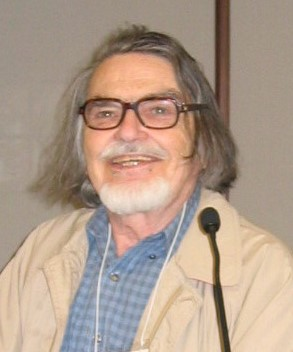
\includegraphics[scale=0.4]{img/Lambek.eps}
 \captionsetup{labelformat=empty}
 \caption{兰贝克(Joachim Lambek) 1922 - 2014}
 \label{fig:Lambek}
\end{figure}
%\end{wrapfigure}

\index{兰贝克定理}
1968年,兰贝克(Lambek)最早指出$i$是一个同构映射,并且称初始代数$(I, i)$是函子$\mathbf{F}$的不动点\cite{Lambek-1968}。现在这一事实被称作\textbf{兰贝克定理}。

F-代数中若存在初始代数$(I, i)$,则存在到任何其它代数$(A, f)$的唯一态射。我们把从$I$到$A$的态射记为$\lbb f \rbb$,使得下面的范畴图可交换:

\begin{center}
\begin{tikzpicture}
  \matrix (m) [matrix of math nodes,
               row sep=3em, column sep=3em, minimum width=2em]{
    \mathbf{F} I  & I \\
    \mathbf{F} A  & A \\};
  \path[-stealth]
    (m-1-1) edge node [above] {$i$} (m-1-2)
    (m-1-1) edge node [left] {$\mathbf{F} \lbb f \rbb$} (m-2-1)
    (m-1-2) edge node [right] {$\lbb f \rbb$}  (m-2-2)
    (m-2-1) edge node [below] {$f$} (m-2-2);
\end{tikzpicture}
\end{center}

\[
  \text{若} h = \lbb f \rbb \text{,当且仅当} h \circ i = f \circ \mathbf{F}(h)
\]

\index{向下态射(catamorphism)}
我们称箭头$\lbb f \rbb$为\textbf{向下态射}(catamorphism,来自希腊语$\kappa \alpha \kappa \alpha$,意思是向下)。它两侧的括号“$\lbb \rbb$”像一对香蕉,因此被称为“香蕉括号”。

向下态射的强大之处在于,它那能把一个非递归结构上的函数$f$,转换为在递归结构上的函数$\lbb f \rbb$。从而构造复杂的递归计算。我们仍然用自然数来举例子。

自然数函子$\mathbf{NatF}$是非递归的,而其起始代数自然数$\mathbf{Nat}$的定义是递归的:

\begin{lstlisting}
data NatF A = ZeroF | SuccF A

data Nat = Zero | Succ Nat
\end{lstlisting}

所以箭头$\mathbf{NatF} A \arrowto{f} A$是非递归的。一个$cata$(向下态射)能够从$f$构造出在递归的$\mathbf{Nat}$上进行计算的箭头$\mathbf{Nat} \to A$。所以$cata$的类型应为:

\[
(\mathbf{NatF} A \arrowto{f} A) \arrowto{cata} (\mathbf{Nat} \to A)
\]

所以(克里化的)$cata(f)$应该能够作用于$\mathbf{Nat}$的两种值$Zero$或者$Succ\ n$。我们可以根据这点定义出$cata$函数:

\[
\begin{array}{l}
cata\ f\ Zero = f\ ZeroF \\
cata\ f\ (Succ\ n) = f (SuccF\ (cata\ f\ n)) \\
\end{array}
\]

这一定义的第一行处理递归的边界情况。针对$\mathbf{Nat}$的零值$Zero$,我们转而用$f$对$\mathbf{NatF}A$的零值$Zero$求值;对于递归情况,也就是$\mathbf{Nat}$的值$Succ\ n$,我们先递归地用$cata\ f\ n$求出类型为$A$的值$a$,然后用$SuccF\ a$将其转化为$\mathbf{NatF}A$类型的值,最后再把$f$作用于其上。这个自然数的向下态射对于任何携带对象$A$都成立,它是非常通用的。我们进一步举两个具体的例子。第一个例子是将任何$\mathbf{Nat}$的值转换回$Int$。

\lstset{frame=single}
\begin{lstlisting}[style=Haskell]
toInt :: Nat -> Int
toInt = cata eval where
  eval :: NatF Int -> Int
  eval ZeroF = 0
  eval (SuccF x) = x + 1
\end{lstlisting}

这样$toInt\ Zero$会得到0,而$toInt\ (Succ\ (Succ\ (Succ\ Zero)))$会得到3。为了方便验证,可以再定义一个辅助函数:

\begin{lstlisting}[style=Haskell]
fromInt :: Int -> Nat
fromInt 0 = Zero
fromInt n = Succ (fromInt (n-1))
\end{lstlisting}

对于任何整数$n$,有$n = (toInt \circ fromInt)\ n$。这个例子看起来很平常,我们来看第二个关于斐波那契数列的例子。

\begin{lstlisting}[style=Haskell]
toFib :: Nat -> (Integer, Integer)
toFib = cata fibAlg where
  fibAlg :: NatF (Integer, Integer) -> (Integer, Integer)
  fibAlg ZeroF = (1, 1)
  fibAlg (SuccF (m, n)) = (n, m + n)
\end{lstlisting}

我们特意将此前定义的函数$fib$改名为$fibAlg$,意思是说,从斐波那契的代数关系(非递归的),我们通过向下态射获得了递归计算斐波那契数列的能力。这样$toFib\ Zero$会得到数对$(1, 1)$,而$toFib\ (Succ\ (Succ\ (Succ\ Zero)))$会得到数对$(3, 5)$。下面的辅助函数,可以计算第$n$个斐波那契数。

\[
fibAt = fst \circ toFib \circ fromInt
\]

事实上,对于任何满足皮亚诺公理的类自然数代数结构$(A, c + f)$,我们都可以利用向下态射和初始代数$(\mathbf{Nat}, zero + succ)$,得到能够进行递归计算的$\lbb c + f \rbb$\footnote{我们用符号$\lbb c + f \rbb$是因为$\lbb [c, f] \rbb$看起来有太多重括号了。}。我们接下来证明这一点。考虑下面的范畴图。

\begin{center}
\begin{tikzpicture}
  \matrix (m) [matrix of math nodes,
               row sep=3em, column sep=5em, minimum width=2em]{
    \mathbf{NatF} \mathbf{Nat}  & \mathbf{Nat} \\
    \mathbf{NatF} A  & A \\};
  \path[-stealth]
    (m-1-1) edge node [above] {$[zero, succ]$} (m-1-2)
    (m-1-1) edge node [left] {$\mathbf{NatF}(h)$} (m-2-1)
    (m-1-2) edge node [right] {$h$}   (m-2-2)
    (m-2-1) edge node [below] {$[c, f]$} (m-2-2);
\end{tikzpicture}
\end{center}

由于向下态射使得这个范畴图可交换。

\[
\begin{array}{rll}
            & h \circ [zero, succ] = [c, f] \circ \mathbf{NatF}(h) & \text{可交换} \\
\Rightarrow & h \circ [zero, succ] = [c, f] \circ (id + h) & \text{多项式函子} \\
\Rightarrow & h \circ [zero, succ] = [c \circ id, f \circ h] & \text{右侧用余积的吸收律} \\
\Rightarrow & [h \circ zero, h \circ succ] = [c, f \circ h] & \text{左侧用余积的融合律} \\
\Rightarrow &
  \begin{cases}
    h \circ zero = c \\
    h \circ succ = f \circ h \\
  \end{cases} & \\
\Rightarrow &
  \begin{cases}
    h\ Zero = c \\
    h\ (Succ\ n) = f(h(n))
  \end{cases} & \\
\Rightarrow &
  \begin{cases}
    h(0) = c \\
    h(n + 1) = f(h(n))
  \end{cases} & \\
\end{array}
\]

这恰恰是自然数叠加的定义:

\[
  h = foldn(c, f)
\]

也就是说,自然数上的向下态射$\lbb c + f \rbb = foldn(c, f)$。因此,对于斐波那契数列,我们可以用

\[
\lbb fibAlg \rbb = \lbb start + next \rbb = foldn(start, next)
\]

来进行代数计算。读到这里,大家会有一种转了一大圈又回到了第一章的感觉。这是一种认知的螺旋上升。第一章中,我们是用归纳和抽象的方法得到了这个结论,现在,我们从更高的层面,把抽象的规律应用到具体的问题上得到了同样的结论。

\subsubsection{代数数据类型}

使用初始F-代数,我们可以定义更多的代数数据类型。本小节我们介绍列表和二叉树的例子。

\begin{example}
在第一章中,我们给出的列表定义为:

\lstset{frame=none}
\begin{lstlisting}
data List A = Nil | Cons A (List A)
\end{lstlisting}

而相应的非递归函子为:

\begin{lstlisting}
data ListF A B = NilF | ConsF A B
\end{lstlisting}

实际上$\mathbf{List}$是函子$\mathbf{ListF}$的不动点。我们可以这样验证。令$B' = \mathbf{ListF}\ A\ B$,然后递归地应用到自己上无穷多次。把这个结果叫做$\mathbf{Fix}\ (\mathbf{ListF}\ A)$:

\[
\begin{array}{rcll}
\mathbf{Fix}\ (\mathbf{ListF}\ A)
& = & \mathbf{ListF}\ A (\mathbf{Fix}\ (\mathbf{ListF}\ A)) & \text{不动点的定义} \\
& = & \mathbf{ListF}\ A\ (\mathbf{ListF}\ A\ (...)) & \text{展开} \\
& = & NilF\ |\ ConsF\ A\ (\mathbf{ListF}\ A\ (...)) & \mathbf{ListF}\ A\ \text{的定义} \\
& = & NilF\ |\ ConsF\ A\ (\mathbf{Fix}\ (\mathbf{ListF}\ A)) & \text{反向用不动点} \\
\end{array}
\]

和$\mathbf{List}\ A$的定义对比,我们有:

\[
\mathbf{List}\ A = \mathbf{Fix}\ (\mathbf{ListF}\ A)
\]

在$\mathbf{ListF}$这个函子下,固定$A$,对于任何携带对象$B$可以定义箭头

\[
\mathbf{ListF}\ A\ B \arrowto{f} B
\]

这样就构成了列表的F-代数。并且我们知道初始代数就是$(List, [nil, cons])$。所以就会有向下态射。

\begin{center}
\begin{tikzpicture}
  \matrix (m) [matrix of math nodes,
               row sep=3em, column sep=5em, minimum width=2em]{
    \mathbf{ListF}\ A\ (\mathbf{List}\ A)  & (\mathbf{List}\ A) \\
    \mathbf{ListF}\ A\ B & B \\};
  \path[-stealth]
    (m-1-1) edge node [above] {$[nil, cons]$} (m-1-2)
    (m-1-1) edge node [left] {$(\mathbf{ListF}\ A)(h)$} (m-2-1)
    (m-1-2) edge node [right] {$h$}   (m-2-2)
    (m-2-1) edge node [below] {$[c, f]$} (m-2-2);
\end{tikzpicture}
\end{center}

如果我们有一个非递归的计算$f$,就可以利用向下态射构成针对递归列表的计算。

\lstset{frame=single}
\begin{lstlisting}[style=Haskell]
cata :: (ListF a b -> b) -> (List a -> b)
cata f Nil = f NilF
cata f (Cons x xs) = f (ConsF x (cata f xs))
\end{lstlisting}

例如,可以定义计算列表长度的代数规则:

\begin{lstlisting}[style=Haskell]
len :: (List a) -> Int
len = cata lenAlg where
  lenAlg :: ListF a Int -> Int
  lenAlg NilF = 0
  lenAlg (ConsF _ n) = n + 1
\end{lstlisting}

这样$len\ Zero$会得到0,而$len\ (Cons\ 1\ (Cons\ 1\ Zero))$则得到2。可以定义一个辅助函数从中括弧简记法转换为$List$:

\begin{lstlisting}
fromList :: [a] -> List a
fromList [] = Nil
fromList (x:xs) = Cons x (fromList xs)
\end{lstlisting}

这样就可以通过$len (fromList [1, 1, 2, 3, 5, 8])$计算列表的长度。

通过改变代数规则$f$,还可以得到其它针对列表的计算。下面的例子把列表中所有的元素累加起来:

\begin{lstlisting}
sum :: (Num a) => (List a) -> a
sum = cata sumAlg where
  sumAlg :: (Num a) => ListF a a -> a
  sumAlg NilF = 0
  sumAlg (ConsF x y) = x + y
\end{lstlisting}

我们接下来利用列表的范畴图证明,列表的向下态射本质上就是叠加计算$foldr$。
列表函子本质上是多项式函子$\mathbf{ListF}\ A\ B = 1 + A \times B$。由于范畴图可交换,所以:

\[
\begin{array}{rll}
            & h \circ [nil, cons] = [c, f] \circ (\mathbf{ListF}\ A)(h) & \text{可交换} \\
\Rightarrow & h \circ [nil, cons] = [c, f] \circ (id + (id \times h)) & \text{多项式函子} \\
\Rightarrow & h \circ [nil, cons] = [c \circ id, f \circ (id \times h)] & \text{右侧用余积的吸收律} \\
\Rightarrow & [h \circ nil, h \circ cons] = [c, f \circ (id \times h)] & \text{左侧用余积的融合律} \\
\Rightarrow &
  \begin{cases}
    h \circ nil = c \\
    h \circ cons = f \circ (id \times h) \\
  \end{cases} & \\
\Rightarrow &
  \begin{cases}
    h\ Nil = c \\
    h\ (Cons\ a\ x) = f(a, h(x))
  \end{cases} & \\
\end{array}
\]

这恰恰是列表叠加的定义:

\[
  h = foldr(c, f)
\]

也就是说,列表F-代数的向下态射$\lbb c + f \rbb = foldr(c, f)$。因此,求长度的
运算是$foldr(0, (a, b) \mapsto b + 1)$,累加的运算是$foldr(0, +)$。
\end{example}

\begin{example}
在第二章中,我们定义了二叉树的类型为:

\lstset{frame=none}
\begin{lstlisting}
data Tree A = Nil | Br A (Tree A) (Tree A)
\end{lstlisting}

所有类似二叉树的结构也可以通过F-代数来描述。首先定义函子:

\begin{lstlisting}
data TreeF A B = NilF | BrF A B B
\end{lstlisting}

携带对象是$B$,而初始代数是$(\mathbf{Tree}\ A, [nil, branch])$。我们把证明作为本小节的练习。这样二叉树的向下态射表示为如下范畴图:

\begin{center}
\begin{tikzpicture}
  \matrix (m) [matrix of math nodes,
               row sep=3em, column sep=5em, minimum width=2em]{
    \mathbf{TreeF}\ A\ (\mathbf{Tree}\ A)  & (\mathbf{Tree}\ A) \\
    \mathbf{TreeF}\ A\ B & B \\};
  \path[-stealth]
    (m-1-1) edge node [above] {$[nil, branch]$} (m-1-2)
    (m-1-1) edge node [left] {$(\mathbf{TreeF}\ A)(h)$} (m-2-1)
    (m-1-2) edge node [right] {$h$}   (m-2-2)
    (m-2-1) edge node [below] {$[c, f]$} (m-2-2);
\end{tikzpicture}
\end{center}

我们可以定义二叉树的向下态射函数。它接受一个F-代数的箭头$\mathbf{TreeF}\ A\ B \arrowto{f} B$,返回一个从$\mathbf{Tree}\ A \to B$的函数:

\[
\begin{array}{l}
cata : (\mathbf{TreeF}\ A\ B \to B) \to (\mathbf{Tree}\ A \to B) \\
cata\ f\ Nil = f\ NilF \\
cata\ f\ (Br\ k\ l\ r) =f\ (BrF\ k\ (cata\ f\ l)\ (cata\ f\ r)) \\
\end{array}
\]

如果定义了一个将二叉树中元素累加起来的代数运算,就可以利用向下态射递归地应用到任意二叉树上:

\[
\begin{array}{l}
sum : \mathbf{Tree}\ A \to A \\
sum = cata \circ sumAlg \\
\text{其中:}
      \begin{cases}
        sumAlg : \mathbf{TreeF}\ A\ B \to B \\
        sumAlg\ NilF = 0_{B} \\
        sumAlg\ (Br\ k\ l\ r) = k + l + r \\
      \end{cases} \\
\end{array}
\]

接下来,我们证明二叉树的向下态射就相当于二叉树的叠加操作$foldt$。固定对象$A$,二叉树的函子$\mathbf{TreeF}\ A\ B$是携带对象$B$的一个多项式函子。即:$\mathbf{TreeF}\ A\ B = 1 + (A \times B \times B)$,对于箭头$h$,为:$(\mathbf{TreeF}\ A)(h) = id + (id_A \times h \times h)$。

由于上面的范畴图可交换,所以有:

\[
\begin{array}{rll}
            & h \circ [nil, branch] = [c, f] \circ (\mathbf{TreeF}\ A)(h) & \text{可交换} \\
\Rightarrow & h \circ [nil, branch] = [c, f] \circ (id + (id_A \times h \times h)) & \text{多项式函子} \\
\Rightarrow & h \circ [nil, branch] = [c \circ id, f \circ (id_A \times h \times h)] & \text{右侧用余积的吸收律} \\
\Rightarrow & [h \circ nil, h \circ branch] = [c, f \circ (id_A \times h)] & \text{左侧用余积的融合律} \\
\Rightarrow &
  \begin{cases}
    h \circ nil = c \\
    h \circ branch = f \circ (id_A \times h \times h) \\
  \end{cases} & \\
\Rightarrow &
  \begin{cases}
    h\ Nil = c \\
    h\ (Br\ k\ l\ r) = f(k, h(l), h(r))
  \end{cases} & \\
\end{array}
\]

这恰恰是二叉树叠加的定义$h = foldt(c, f)$,其中:

\[
\begin{cases}
foldt\ c\ h\ Nil = c \\
foldt\ c\ h\ (Br\ k\ l\ r) = h(k, foldt\ c\ h\ l, foldt\ c\ h\ r) \\
\end{cases}
\]

因此,累加二叉树中元素的运算可以用叠加表示为$foldt(0_B, (\bullet + \bullet + \bullet))$。
\end{example}

\begin{Exercise}
\Question{对二叉树函子$\mathbf{TreeF}\ A\ B$,固定$A$,利用不动点验证$(\mathbf{Tree}\ A, [nil, branch])$是初始代数。}
\end{Exercise}

\section{小节}

本章介绍了范畴论中最基本的概念,包括范畴、函子、自然变换。并且还介绍了积和余积、起始对象和终止对象、幂以及F-代数这些工具来构造较为复杂的代数结构。作为本章的结尾,我们来解读一段Haskell标准库中关于叠加的代码\cite{Haskell-foldable}。通常我们认为列表的叠加操作可以这样写:

\lstset{language=Haskell, frame=single}
 \begin{lstlisting}
foldr f z [] = z
foldr f z (x:xs) = f x (foldr f z xs)
\end{lstlisting}

但实际上,今天的标准库用范畴的语言这样写:

\lstset{frame=single}
\begin{lstlisting}
foldr f z t = appEndo (foldMap (Endo . f) t) z
\end{lstlisting}

所有的这一切的背后都是为了抽象,为了使得$foldr$能跳出列表。在传统的列表叠加定义中,$f$是一个二元操作,如果我们把它改写为$\oplus$,把$z$改写为单位元$e$,根据这个定义,$foldr\ (\oplus)\ e\ [a, b, c]$就可以展开成为:

\[
a \oplus (b \oplus (c \oplus e))
\]

这让我们联想到幺半群,$foldr$相当于在幺半群上重复进行二元操作。在Haskell的抽象幺半群定义中,除了单位元和二元操作外,还定义了将一列元素“累加”的操作。用我们的$\oplus$和$e$符号,这个定义相当于:

\[
\begin{array}{l}
concat_M : [M] \to M \\
concat_M = foldr\ (\oplus)\ e \\
\end{array}
\]

在Haskell中这个函数的名字叫做\texttt{mconcat}。它的意思是说,对于任何幺半群$M$,$concat$可以将一个$M$中元素的列表,通过二元运算和单位元叠加计算到一起。例如字符串可以看作是幺半群,单位元是空串,而二元运算是连接。所以$concat_M$ \texttt{["Hello", "String" "Monoid"]}就得到:

\begin{verbatim}
"Hello" ++ ("String" ++ ("Monoid" ++ "")) = "HelloStringMonoid"
\end{verbatim}

现在我们可以对任何幺半群元素进行累加了。但能否让它变得更通用呢?如果有一列元素,它们虽然不是幺半群中的元素,但是如果我们能将它们转换为幺半群,就仍然可以进行累加。将某一类型的列表映射为幺半群列表恰巧就是函子的行为,确切地说我们把箭头$A \arrowto{g} M$,通过列表函子“举”到$\mathbf{List}(g)$。然后再执行累加:

\begin{center}
\begin{tikzpicture}
  \matrix (m) [matrix of math nodes,
               row sep=2em, column sep=5em, minimum width=2em]{
     \lbrack A \rbrack & \lbrack M \rbrack & M\\
     A   &  M  & \\};
  \path[-stealth]
    (m-1-1) edge node [above] {$fmap\ g$} (m-1-2)
    (m-2-1) edge node [above] {$g$} (m-2-2)
    (m-2-1) edge node [left] {$\mathbf{List}$} (m-1-1)
    (m-2-2) edge node [right] {$\mathbf{List}$} (m-1-2)
    (m-1-2) edge node [above] {$concat$} (m-1-3);
\end{tikzpicture}
\end{center}

\[
\begin{array}{l}
foldMap : (A \to M) \to [A] \to M \\
foldMap\ g = concat_M \circ fmap\ g
\end{array}
\]

可是美中不足的是,对于任何传入$foldr$的二元组合函数$f : A \to B \to B$,如果$B$不是幺半群,我们仍然无法进行叠加。现在考虑$f$的克里化形式$f : A \to (B \to B)$,我们发现以箭头$B \to B$为对象,可以组成一个幺半群。其中单位元是恒等箭头$id$,而二元运算是函数组合。为此,我们把这种$B \to B$的箭头通过函子封装成一个类型(集合):

\lstset{frame=none}
\begin{lstlisting}[style=Haskell]
newtype Endo B = Endo (B -> B)
\end{lstlisting}

并且定义一个函数,从$\mathbf{Endo}B \arrowto{appEndo} B$:

\[
appEndo(Endo\ a) = a
\]

然后我们规定$\mathbf{Endo}$是一个幺半群,单位元是$id$,二元运算是函数组合。在Haskell中,这相当于以下代码:

\lstset{frame=single}
\begin{lstlisting}[style=Haskell]
instance Monoid Endo where
    mempty = Endo id
    Endo f `mappend` Endo g = Endo (f . g)
\end{lstlisting}

现在任给一个二元组合函数$f$,我们都可以把它利用$foldMap$叠加到$Endo$幺半群上去了:

\[
\begin{array}{l}
foldCompose : (A \to (B \to B)) \to [A] \to \mathbf{Endo}B \\
foldCompose\ f = foldMap\ (Endo . f)
\end{array}
\]

这样如果计算$foldCompose\ f\ [a, b, c]$则展开为:

\[
\begin{array}{cl}
  & Endo(f\ a) \oplus (Endo(f\ b) \oplus (Endo(f\ c) \oplus Endo(id))) \\
= & Endo(f\ a \oplus (f\ b \oplus (f\ c \oplus id))
\end{array}
\]

下面是一个具体的例子

\[
\begin{array}{cl}
            & foldCompose\ (+)\ [1, 2, 3] \\
\Rightarrow & foldMap\ (Endo \circ (+))\ [1, 2, 3] \\
\Rightarrow & concat_M\ (fmap (Endo \circ (+)))\ [1, 2, 3] \\
\Rightarrow & concat_M\ (fmap Endo\ [(+1), (+2), (+3)]) \\
\Rightarrow & concat_M\ [Endo\ (+1), Endo\ (+2), Endo\ (+3)] \\
\Rightarrow & Endo\ ((+1) \circ (+2) \circ (+3)) \\
\Rightarrow & Endo\ (+6) \\
\end{array}
\]

所以,最后一步我们要把$Endo$中的结果取回。具体到这个例子,就是用$appEndo$把$(+6)$拿出,然后把它应用到传入$foldr$的初始值$z$上:

\[
\begin{array}{rcll}
foldr\ f\ z\ xs
  & = & appEndo\ (foldCompose\ f\ xs)\ z & \\
  & = & appEndo\ (foldMap\ (Endo \circ f)\ xs)\ z \\
\end{array}
\]

这就是我们看到的$foldr$定义。在Haskell中,还专门定义了类型$Foldable$,对任意数据结构,使用者可以选择实现$foldMap$或者$foldr$。具体请参见本章附录。

\section{扩展阅读}

限于篇幅,我们不可能仅仅在一章中完成范畴论的介绍。本章的内容不过是冰山的一个小角。范畴论的核心精神是抽象。初始对象和终止对象,积和余积这些对偶的概念,它们本质上可以进一步抽象到更高层次的对偶——极限(limits)和余极限(colimits)。我们没能介绍伴随(junction)的概念,没能介绍米田定理(Yoneda lemma),也没有能够解读单子。我希望这一章能够起到抛砖引玉的作用,引导读者去阅读和了解更多的内容。范畴论的创始人之一麦克兰恩的编写的教材\cite{Mac-Lane-1998}是这个领域的经典。其目标读者是数学家,普通读者读起来有些艰深。西蒙森的《范畴论引论》\cite{Simmons2011}和史密斯的\cite{PeterSmith2018}更适合初学者。对于有编程背景的读者,迈尔维斯基的《程序员的范畴论》\cite{Milewski2018}是本不错的参考书。里面配有很多Haskell示例代码和一些C++的类比实现。但是这本书仅仅在集合全函数范畴(确切地说是Hask范畴)内讨论。伯德的《编程中的代数》\cite{Bird97}更加全面地介绍了编程中的范畴原理。

% limits/colimits, 伴随,米田定理

\section{附录:例子代码}

函子的定义:

\lstset{frame=single}
\begin{lstlisting}[style=Haskell]
class  Functor f  where
    fmap        :: (a -> b) -> f a -> f b
\end{lstlisting}

Maybe函子的定义:

\begin{lstlisting}
instance  Functor Maybe  where
    fmap _ Nothing       = Nothing
    fmap f (Just a)      = Just (f a)
\end{lstlisting}

使用Maybe搜索二叉搜索树,并将结果转换成二进制:

\begin{lstlisting}[style=Haskell]
lookup Nil _ = Nothing
lookup (Node l k r) x | x < k = lookup l x
                      | x > k = lookup r x
                      | otherwise = Just k

lookupBin = (fmap binary) . lookup
\end{lstlisting}

二元函子的定义:

\begin{lstlisting}
class Bifunctor f where
  bimap :: (a -> c) -> (b -> d) -> f a b -> f c d
\end{lstlisting}

积函子和余积函子的定义:

\begin{lstlisting}
instance Bifunctor (,) where
  bimap f g (x, y) = (f x, g y)

instance Bifunctor Either where
  bimap f _ (Left a) = Left (f a)
  bimap _ g (Right b) = Right (g b)
\end{lstlisting}

$curry$及其反向变换$uncurry$的定义:

\begin{lstlisting}
curry       :: ((a, b) -> c) -> a -> b -> c
curry f x y =  f (x, y)

uncurry     :: (a -> b -> c) -> ((a, b) -> c)
uncurry f (x, y) =  f x y
\end{lstlisting}

幺半群的定义:

\begin{lstlisting}
class Semigroup a => Monoid a where
    mempty  :: a

    mappend :: a -> a -> a
    mappend = (<>)

    mconcat :: [a] -> a
    mconcat = foldr mappend mempty
\end{lstlisting}

可叠加类型(Foldable)的定义:

\begin{lstlisting}
newtype Endo a = Endo { appEndo :: a -> a }

class Foldable t where
    foldr :: (a -> b -> b) -> b -> t a -> b
    foldr f z t = appEndo (foldMap (Endo . f) t) z

    foldMap :: Monoid m => (a -> m) -> t a -> m
    foldMap f = foldr (mappend . f) mempty
\end{lstlisting}

\ifx\wholebook\relax \else
\begin{thebibliography}{99}

\bibitem{Dieudonne1987}
[法]让$\cdot$迪厄多内 著,沈用欢 译 ``当代数学,为了人类心智的荣耀''. 上海教育出版社. 2000年3月. ISBN: 7532063062

\bibitem{Monad-Haskell-Wiki}
Haskell Wiki. ``Monad''. \url{https://wiki.haskell.org/Monad}

\bibitem{Wiki-Eilenberg}
Wikipedia. ``塞缪尔$\cdot$艾伦伯格''. \url{https://en.wikipedia.org/wiki/Samuel_Eilenberg}

\bibitem{Wiki-Mac-Lane}
Wikipedia. ``桑德斯$\cdot$麦克兰恩''. \url{https://en.wikipedia.org/wiki/Saunders_Mac_Lane}

\bibitem{Simmons2011}
Harold Simmons. ``An introduction to Category Theory''.  Cambridge University Press; 1 edition, 2011. ISBN: 9780521283045

\bibitem{Wiki-Hoare}
Wikipedia. ``Tony Hoare''. \url{https://en.wikipedia.org/wiki/Tony_Hoare}

\bibitem{Wadler-1989}
Wadler Philip. ``Theorems for free!''. Functional Programming Languages and Computer Architecture, pp. 347-359. Asociation for Computing Machinery. 1989.

\bibitem{Milewski2018}
Bartosz Milewski. ``Category Theory for Programmers''. \url{https://bartoszmilewski.com/2014/10/28/category-theory-for-programmers-the-preface/}

\bibitem{Bird97}
Richard Bird, Oege de Moor. ``Algebra of Programming''. University of Oxford, Prentice Hall Europe. 1997. ISBN: 0-13-507245-X.

\bibitem{PeterSmith2018}
Peter Smith. ``Category Theory - A Gentle Introduction''. \url{http://www.academia.edu/21694792/A_Gentle_Introduction_to_Category_Theory_Jan_2018_version_}

\bibitem{Wiki-Exponentials}
Wikipedia. ``Exponential Object''. \url{https://en.wikipedia.org/wiki/Exponential_object}

\bibitem{Manes-Arbib-1986}
Manes, E. G. and Arbib, M. A. ``Algebraic Approaches to Program Semantics''. Texts and Monographs in Computer Science. Springer-Verlag. 1986.

\bibitem{Lambek-1968}
Lambek, J. ``A fixpoint theorem for complete categories''. Mathematische Zeischrift, 103, pp.151-161. 1968.

\bibitem{Haskell-foldable}
Wikibooks. ``Haskell/Foldable''.  \url{https://en.wikibooks.org/wiki/Haskell/Foldable}

\bibitem{Mac-Lane-1998}
Mac Lane. ``Categories for working mathematicians''. Springer-Verlag. 1998. ISBN: 0387984038.

\end{thebibliography}

\expandafter\enddocument
%\end{document}

\fi
